\lstset{basicstyle=\footnotesize\sffamily,language=Java,moreemph={end},emphstyle=\bfseries,commentstyle=\itshape,frame=single}
% v\'erifier preuve
% exemple complet
% ATTENTION a la decomposition : pr\'eservation du comportement du
% composant d\'ecompos\'e

Les automates FIDL  d\'etaill\'es au chapitre pr\'ec\'edent
constituent la brique de base de la mod\'elisation des entit\'es
dans le mod\`ele d'architecture de composants sur lequel nous
travaillons. Naus n'avons toutefois encore rien pr\'ecis\'e de la
formalisation de ces entit\'es et de la mani\`ere dont elles peuvent
s'agencer et dont une sp\'ecification d\'ecrit leur comportement.   

Ce chapitre pr\'esente donc la s\'emantique formelle des
\'el\'ements mod\'elis\'es : interfaces, composants, connexions,
assemblages et composites. Par s\'emantique, nous entendons
d\'efinir le \emph{sens}  pr\'ecis de chacune des constructions
syntaxiques qu'il est possible d'\'ecrire selon la grammaire
\textsf{FIDL}. Ce sens est d\'efini en termes de \emph{langages} clos
par pr\'efixes appel\'es aussi \emph{ensembles de traces}, sur des alphabets dont
les lettres poss\`edent une structure particuli\`ere. La premi\`ere
partie d\'ecrit la s\'emantique des \'el\'ements atomiques d'un
mod\`ele : \'ev\'enements, interfaces, composants primitifs. La
deuxi\`eme partie s'attachera \`a d\'efinir le comportement d'un
syst\`eme lorsqu'il est constitu\'e de plusieurs \'el\'ements mis
en relation. Nous d\'emontrerons en particulier un r\'esultat de
pr\'eservation de la correction des composants lors de leur
composition. La derni\`ere partie sera consacr\'ee aux propri\'et\'es
de sous-typage et d'h\'eritage et \`a la mani\`ere dont celles-ci
sont d\'efinies dans notre mod\`ele.
  
\section{\'El\'ements atomiques}
\label{section-semantique}

\`A partir de la definition de la structure de l'alphabet, c'est \`a
dire des \'ev\'enements, 
nous d\'efinissons les alphabets et langages associ\'es \`a une
interface et \`a un composant. Ces \'ev\'enements pr\'esentent la
particularit\'e  d'encapsuler dans chaque lettre la
connectique du syst\`eme dans lequel est produit l'\'ev\'enement
sous la forme de variables identifiant pr\'ecis\'ement l'emetteur
et le r\'ecepteur d'un message. Au fur et \`a mesure du processus de
composition, ces variables sont instanci\'ees avec les identit\'es
concr\`etes des \'el\'ements qu'elles repr\'esentent.

\subsection{\'Ev\'enements}

Nous pr\'ecisons dans cette section la structure de l'ensemble ${\cal
  X}$ (voir chapitre
  \ref{cha:automates-fidl}, section \ref{sec:alphabet}) dans le cas
  des mod\'eles de composants. Rappelons que $\cal X$ est l'ensemble
  des \emph{enveloppes} des lettres reconnues par un automate FIDL. 
Ces enveloppes sont d\'enomm\'ees ici \emph{types
  d'\'ev\'enements}. Chacun repr\'esente une partie d'un \emph{message}
  envoy\'e d'un \'emetteur vers run r\'ecepteur. 

\begin{definition}[\'Ev\'enement]
\label{sec:evenements}    Un \'ev\'enement est un n-uplet
    $(\gamma_1,\varrho_1,\gamma_2,\varrho_2,k,m,v)$
    o\`u :
\begin{itemize}
  \item $\gamma_1,\varrho_1,\gamma_2,\varrho_2$ identifient  une
    connexion, $\gamma_1,\gamma_2$ 
    \'etant respectivement l'identit\'e des composants client et
    serveur  et $\varrho_1,\varrho_2$ identifiant les ports
    connect\'es dans les composants respectifs ;
  \item $k \in
    \{\mathtt{call},\mathtt{return}, \mathtt{exception},\mathtt{async}\}$
    le \emph{genre} de l'\'ev\'enement, respectivement un appel de m\'ethode,
    un retour d'appel, une exception ou un message asynchrone ;
  \item $m$ le nom de l'\'ev\'enement, qui peut \^etre un nom de m\'ethode
    ou de type d'\'ev\'enement. \`A chaque nom d'\'ev\'enement $m$ est
    attach\'e une arit\'e $ar(m)$ et une signature qui est un
    n-uplet de types $(T_1,\dots, T_{ar(m)}$  ;
    %%   \item $(x_1,x_2,\dots,x_n)$ le \emph{corps} du message, un n-uplet de valeurs et de variables
%%   tel que : $\forall i, 1\leq i\leq n, x_i\in {\cal V} \cup {\cal
%%   D}$. Dans le cas des messages $\mathtt{exception}$, on a $\vec{x} =
%%   (E,\bar{y})$ o\`u $E$ est le type de l'exception et $\bar{y}$ le
%%   n-uplet de valeurs et de variables correspondant \`a la structure
%%   de $E$ ;
  \item $v \in \{\mathtt{emit},\mathtt{receive}\}$ le \emph{point de
  vue} sur l'\'ev\'enement, respectivement une \emph{\'emission} et
  une \emph{r\'eception}.
\end{itemize}
\end{definition}

%% exemples 
L'ensemble de tous les messages est not\'e comme pr\'ec\'edemment
${\cal E}$ et il est construit \`a partir de la structure des
\'ev\'enements et d'un contenu d\'ependant de l'arit\'e et de la
signature des messages. Un message est not\'e
$(\gamma_1,\varrho_1,\gamma_2,\varrho_2,k,m,\vec{x},v)$ o\`u
$\vec{x}$ est le \emph{contenu} du message et les autres
\'el\'ements du n-uplet son enveloppe. Le nombre et le type des \'el\'ements du
vecteur $\vec{x}$ d\'ependent de la signature associ\'ee \`a $m$.

L'ensemble de tous les \emph{messages clos}, c'est
\`a dire tous les messages dont le corps ne contient que des
litt\'eraux, est not\'e  $\bar{\cal E}$ :
$$\bar{\cal E} =\{
(\gamma_1,\varrho_1,\gamma_2,\varrho_2,k,m,(x_1,x_2,\dots,x_{ar(m)}),v) \in {\cal E} \mid
\forall i, 1\leq i \leq ar(m), x_i \in m[i]\}$$
et l'ensemble des \emph{messages abstraits}, not\'e  ${\cal E}_\lambda$ :
 $${\cal E}_\lambda = \{
(\gamma_1,\varrho_1,\gamma_2,\varrho_2,k,m,v) \mid \exists
(\gamma_1,\varrho_1,\gamma_2,\varrho_2,k,m,\vec{x},v) \in {\cal
  E}\},$$ c'est \`a dire l'ensemble des messages en ne
consid\'erant que leur enveloppe. 

On d\'efinit $h_\lambda:{\cal
  E}\rightarrow \cal{E}_\lambda$ le morphisme d'abstraction comme : 
\begin{equation}
\begin{array}{c}
h_\lambda((\gamma_1,\varrho_1,\gamma_2,\varrho_2,k,m,\vec{x},v)) \\
=\\
\left\{\begin{array}{l}
(\gamma_1,\varrho_1,\gamma_2,\varrho_2,\mathtt{return},m,v),\ \mbox{si~}k=\mathtt{exception},\\
(\gamma_1,\varrho_1,\gamma_2,\varrho_2,k,m, v)\
\mbox{sinon}, \\
\end{array}\right.\\
\end{array}\label{eq:def-morph-abst}
\end{equation}
et $\bar{h}:{\cal
  E}\rightarrow \cal{E}$ le \emph{morphisme miroir} :
\begin{equation}
\bar{h} =
h_{\mathtt{emit},\mathtt{receive}}^{\mathtt{receive},\mathtt{emit}}\
.\label{eq:def-morph-mirroir}
\end{equation}

Dans la d\'efinition de  $h_\lambda$, nous abandonnons
la distinction entre les messages de retour d'appels de m\'ethodes et
les messages d'exception, consid\'erant que les exceptions ne sont
qu'un type de retour possible diff\'erent d'un retour normal.. 

Pour simplifier la notation,  nous pourrons \^etre amen\'es \`a d\'enoter le
n-uplet de variables de connexions $(\gamma_1,\varrho_1,\gamma_2,\varrho_2)$ par le
symbole unique $\kappa$ lorsque l'identit\'e des connexions n'est pas n\'ecessaire.

\subsection{Types}
\label{sec:types}

\subsubsection{Interfaces}

Une interface est un \emph{contrat} syntaxique et comportemental sur
un canal de communication entre deux entit\'es d'un syst\`eme. Elle
d\'ecrit l'alphabet des messages  pouvant \^etre
\'echang\'es entre le client et le fournisseur du service
d\'efini par l'interface et le langage associ\'e \`a cet alphabet.

\begin{definition}[Interface]
\label{def:typeinterface}
Une interface $I$ est un couple not\'e $\langle meth(I),
\Tr(I)\rangle$ o\`u $meth(I)$ est un ensemble fini de \emph{m\'ethodes}
et $\Tr(I)$ un langage clos par pr\'efixe sur un certain alphabet
$\ialph(I)$.
\end{definition} 

Toute m\'ethode $m$ appartenant \`a $meth(I)$ est d\'efini par :
\begin{itemize}
  \item son arit\'e $\mathsf{ar}(m)\in \N$ ;
  \item sa signature $\mathsf{sig}(m)$ qui est un vecteur de taille
    $\mathsf{ar}(m)$ dont les \'el\'ements sont des types ${T_1}, \dots ,{T_{ar(m)}}$ ;
  \item ses exceptions, $\mathsf{exceptions}(m)$, un vecteur de
    taille $k$ finie.
\end{itemize}

En supposant que les signatures sont ordonn\'ees selon l'ordre usuel
: d'abord les param\`etres en mode \textbf{in}, ensuite les
\textbf{inout} enfin les param\`etres en mode \textbf{out}, $in(m)$
est l'indice du dernier param\`etre en mode \textbf{in} ou
\textbf{inout} et $out(m)$ est l'indice du premier param\`etre en
mode \textbf{inout} ou \textbf{out}. 

Pour une m\'ethode $m$ de signature $\mathsf{sig}(m)$, on a par ailleurs les ensembles suivants qui
sont d\'efinis :
\begin{itemize}
  \item $ \mathsf{inpar}(m)$ est l'ensemble des vecteurs de param\`etres en mode
    \textbf{in} et \textbf{inout} de la m\'ethode $m$ comprenant des valeurs et
    des variables :
    $$
    \mathsf{inpar}(m) = \{ \vec{x} \in ({\cal V}\cup {\cal D})^{in(m)}
    \mid x[i] \in \mathsf{sig}(m)[i] \} ;
    $$
  \item $\mathsf{outpar}(m)$ l'ensemble des vecteurs de param\`etres en mode
    $inout$- et $out$- de la m\'ethode $m$ comprenant des valeurs et
    des variables ainsi qu'\'eventuellement une valeur de retour de
    la m\'ethode appel\'ee
    $$
    \mathsf{outpar}(m) = \{ \vec{x} \in ({\cal V}\cup {\cal D})^{\mathsf{ar}(m)-out(m)}
    \mid x[i] \in \mathsf{sig}(m)[i+out(m)] \} ;
    $$
  \item $\overline{\mathsf{inpar}}(m)$ l'ensemble des vecteurs de param\`etres en mode $in$- et
    $inout$- de la m\'ethode $m$ ne contenant que des valeurs
    litt\'erales :
    $$
    \overline{\mathsf{inpar}}(m) = \{ \vec{x} \in {\cal D}_{T_1}\times{}
    \dots \times{}{\cal D}_{T_{in(m)}}\} ;
    $$
  \item $\overline{\mathsf{outpar}}(m)$ l'ensemble des vecteurs de param\`etres en mode  $inout$- et 
    $out$- de la m\'ethode $m$ ne contenant que des valeurs
    litt\'erales plus la valeur de retour si
    elle est diff\'erente de \texttt{void} :
    $$
    \overline{\mathsf{outpar}}(m) = \{ \vec{x} \in {\cal D}_{T_{out(m)}}\times{}
    \dots \times{}{\cal D}_{T_{\mathsf{ar}(m)}}\}.
    $$
\end{itemize}

\begin{definition}[Alphabet d'une interface]
\label{def:alphinterface}
L'alphabet d'une interface $I =\langle meth(I),\Tr(I)\rangle$ est
d\'efini comme :
    $$
\begin{array}{rl}
\ialph(I) = \{(\gamma_1,\varrho_1,\gamma_2,\varrho_2,d,m,\vec{x},v) \mid & m \in
meth(I), \\
&(d,\vec{x},v) \in \{\mathtt{call}\} \times{}\overline{\mathsf{inpar}}(m) \times{}
\{\mathtt{receive}\} \\
&\cup \{\mathtt{return}\} \times{}\overline{\mathsf{outpar}}(m) \times{}
\{\mathtt{emit}\} \\
&\cup \{\{\mathtt{exception}\} \times{} (E \times{}{\cal D}_E) \times{}
\{\mathtt{emit}\}, \forall E \in \mathsf{exceptions}(m)\} \}.
\end{array}
$$
\end{definition}


\subsubsection{\'Ev\'enements asynchrones}

Le cas des \'ev\'enements asynchrones est le plus simple : un
\'ev\'enement asynchrone est simplement un n-uplet de valeurs
correctement typ\'ees, c'est \`a dire respectant la structure de la
d\'efinition de l'\'ev\'enement.

\begin{definition}[Type d'\'ev\'enement asynchrone]
\label{def:typeasync}
    Un type d'\'ev\'enement asynchrone $S$ est d\'efini par un
    n-uplet de types  $(T_1,\dots,T_n)$.
L'alphabet associ\'e \`a un \'ev\'enement asynchrone $S$,
    $\ialph(S)$, est d\'efini simplement comme suit :
$$
\ialph(S) = \{(\gamma_1,\varrho_1,\gamma_2,\varrho_2,\mathtt{async},S,(x_1,\dots,x_n),v) \mid
\forall x_i, 1\leq i\leq n, x_i \in {\cal D}_{T_i}\}.
$$
Il est constitu\'e de tous les messages identifi\'es par le nom de
$S$ --- not\'e aussi $S$ --- contenant des valeurs correctes pour la
structure de $S$. Le langage associ\'e \`a un type d'\'ev\'enement
asynchrone est simplement 
$$
\Tr(S) = \ialph(S)^*.
$$
\end{definition}
 
\subsubsection{Composant}

Un composant d\'efinit une entit\'e d'un syst\`eme susceptible
d'\^etre r\'ealis\'ee \`a l'ex\'ecution par une --- ou plusieurs
dans le cas des composites --- instances de composants r\'eels. C'est donc la description d'un
ensemble de services \emph{offerts}  et requis au travers de ports
\emph{identifi\'es} et \emph{typ\'es}, soit par une interface, soit
par un type d'\'ev\'enement asynchrone. 

Nous d\'efinissons donc tout d'abord la notion de port  avant de
d\'efinir la s\'emantique d'un composant.

\begin{definition}[Port]
\label{def:port}
    Un port $p$ est un triplet $(n, t, g)$ o\`u $n$ est le nom du port,
    $t$ son type  qui peut \^etre une interface ou un type
    d'\'ev\'enement asynchrone et $g$ son \emph{genre}
    ($\mathtt{receptacle}, 
    \mathtt{facet}, \mathtt{source}$  ou $\mathtt{sink}$).
\end{definition}

L'alphabet et l'ensemble de traces associ\'es \`a un port
$p=(n,T,g)$, not\'es respectivement $\ialph(p)$ et $\Tr(p)$ sont d\'efinis comme suit :
\begin{description}
  \item[$p=(f,I,\mathtt{facet})$] $\ialph(p) = h_{\varrho_2}^f$ et $\Tr(p)= h_{\varrho_2}^{f}(\Tr(I))$ ;
  \item[$p=(r,I, \mathtt{receptacle})$] $\ialph(p) = h_{\varrho_1}^r$
  et $\Tr(p)= \bar{h}(h_{\varrho_1}^{r}(\Tr(I)))$ ;
  \item[$p=(s,S, \mathtt{source})$] $\ialph(p) = h_{\varrho_1}^s$ et $\Tr(p)= h_{\varrho_1}^{s}(\Tr(S))$  :
  \item[$p=(s,S,\mathtt{sink})$] $\ialph(p) = h_{\varrho_2}^s$ et $\Tr(p)= \bar{h}(h_{\varrho_2}^{s}(\Tr(S)))$.
\end{description}

Un port est simplement une instance nomm\'ee et orient\'ee d'un type d'interface ou
d'\'ev\'enement asynchrone.

\begin{definition}[Composant]
\label{def:typecomp}
Un composant $C$ est d\'efini par un couple $\langle Port(C),\Tr(C)\rangle$
o\`u  $Port(C)$ est un ensemble fini de ports dont les noms sont deux \`a
deux distincts et $\Tr(C)$ un langage clos par pr\'efixe
sur l'alphabet $\ialph(C)$ qui est l'union des alphabets suivants :
\begin{itemize}
  \item $h_{\gamma_2}^{\gamma}(\ialph(p))$ pour chaque facette $p=(f,
    I, \mathtt{facet}) $ de $ Port(C)$ ;
  \item $h_{\gamma_1}^{\gamma}(\ialph(p)))$ pour
    chaque r\'eceptacle $p=(r,
    I, \mathtt{receptacle}) $ de $ Port(C)$ ;
  \item $h_{\gamma_1}^{\gamma}(\ialph(p))$
  pour chaque  source d'\'ev\'enement $p=(s,S,\mathtt{source}) $ de $ Port(C)$ :
  \item $h_{\gamma_2}^{\gamma}(\ialph(p))$
  pour chaque puits d'\'ev\'enement $p=(s,S,\mathtt{sink}) $ de $ Port(C)$.
\end{itemize}
\end{definition}

L'alphabet d'un composant est donc l'alphabet des diff\'erents ports
qui le composent dans lesquels la variable $\gamma_1$  ---
respectivement $\gamma_2$  --- est remplac\'ee par la variable $\gamma$ repr\'esentant
n'importe quelle instance du
composant $C$. 

Pour un composant donn\'e $C$, nous noterons :
\begin{itemize}
  \item $\F(C)=\{(f,I, \mathtt{facet}) \in Port(C)\}$, l'ensemble de
  ses facettes ;
\item   $\R(C)=\{(r,I, \mathtt{receptacle}) \in Port(C)\}$, l'ensemble de
  ses r\'eceptacles ;
\item  $\Source(C)=\{(s,S, \mathtt{source}) \in Port(C)\}$, l'ensemble de
  ses sources ;
\item et $\Sink(C)=\{(s,S, \mathtt{sink}) \in Port(C)\}$, l'ensemble de
  ses puits.
\end{itemize}

On peut alors d\'ecrire une instance particuli\`ere du composant $C$
en instantiant simplement la variable $\gamma$ avec l'identit\'e de
l'instance de composant.

\begin{definition}[Instance de composant]
\label{def:instcomp}
 Une instance du composant  $C = \langle Port(C),\Tr(C) \rangle$ dont
 l'identit\'e est  $c$ est d\'efini simplement par le couple :
$$c = \langle Port(C),h_{\gamma}^{c}(\Tr(C)) \rangle,$$
et son alphabet est :
$$\ialph(c) = h_{\gamma}^{c}(\ialph(C)).$$
\end{definition}

\subsection{Expressions \textsf{FIDL}}

Les comportements des interfaces et des composants sont d\'ecrits au
moyen d'expressions \textsf{FIDL} dont la syntaxe a \'et\'e
introduite partiellement dans la section \ref{sec:grammaire}. Nous
donnons ici le lien entre la d\'efinition formelle des messages et la notation
utilis\'ee (voir tableau \ref{tbl-correspondance-composant}). Notons que l'utilisation de
vecteurs de variables diff\'erents pour les deux \'ev\'enements
induits par une notation appel/retour s'explique par le fait que les
param\`etres \texttt{in} et \texttt{out} peuvent n'\^etre qu'un
sous-ensemble de tous les param\`etres de la m\'ethode, on a donc
pour chaque m\'ethode $m$ et chaque vecteur $\vec{x}$, 
$\vec{y}\in inpar(m)$ et $\vec{z}\in outpar(m)$, et $\vec{x}$ est \og l'union\fg{} des deux
vecteurs. La nature des
param\`etres du vecteur $\vec{x}$ se d\'eduit imm\'ediatement de
son utilisation dans les messages.

\begin{figure}[htbp]
  \centering
\begin{tabular}{|l|l|l|}
\hline
Composant&Notation&\'Ev\'enement\\
\hline
Appel sur r\'eceptacle&$r\rightarrow m(\bar{x})$&$(c,r, \gamma_2, \varrho_2, \mathtt{call}, m, \vec{x}, \mathtt{emit})$\\
Retour correspondant&$r \leftarrow m (\bar{x})$&$(c,r,  \gamma_2, \varrho_2, \mathtt{return}, m, \vec{x}, \mathtt{receive})$\\
Appel/retour sur r\'eceptacle&$r.m(\bar{x})$&$\begin{array}{l}(c,r,
    \gamma_2, \varrho_2, \mathtt{call}, m, \vec{y}, \mathtt{emit})\\ (c,r,  \gamma_2, \varrho_2, \mathtt{return}, m, \vec{z}, \mathtt{receive})\end{array}$\\
Appel re\c{c}u sur facette $f$&$f\rightarrow m (\bar{x})$&$(  \gamma_1, \varrho_1, c,f, \mathtt{call}, m, \vec{x}, \mathtt{receive})$\\
Retour correspondant&$f\leftarrow m(\bar{x})$&$( \gamma_1, \varrho_1,c,f, \mathtt{return}, m, \vec{x}, \mathtt{emit})$\\
Appel/retour sur facette $f$&$f.m(\bar{x})$&$\begin{array}{l}(
    \gamma_1, \varrho_1, c,f, \mathtt{call}, m, \vec{y},
    \mathtt{receive})\\ (\gamma_1, \varrho_1,c,f, \mathtt{return}, m, \vec{z}, \mathtt{emit})\end{array}$\\
Envoi d'\'ev\'enement&$so.[\bar{x}]$&$(c,so, \gamma_2, \varrho_2, \mathtt{event}, Type(so), \vec{x}, \mathtt{emit})$\\
R\'eception d'\'ev\'enement&$si.[\bar{x}]$&$( \gamma_1, \varrho_1,c, si, \mathtt{event}, Type(si), \vec{x}, \mathtt{receive}) $\\ 
\hline
Interface&&\\
\hline
Appel& $\rightarrow m(\bar{x})$&$(\gamma_1, \varrho_1, \gamma_2, \varrho_2, \mathtt{call}, m, \vec{x}, \mathtt{receive})$\\
Retour& $\leftarrow m (\bar{x})$&$(\gamma_1, \varrho_1, \gamma_2, \varrho_2, \mathtt{return}, m, \vec{x}, \mathtt{emit})$\\
Exception& $\leftarrow m (E,\bar{x})$&$(\gamma_1, \varrho_1, \gamma_2, \varrho_2, \mathtt{exception}, m, (E,\bar{x}), \mathtt{emit})$\\
Appel/retour& $m (\bar{x})$&$\begin{array}{l}(\gamma_1, \varrho_1,
    \gamma_2, \varrho_2, \mathtt{call}, m, \vec{y},
    \mathtt{receive})\\ (\gamma_1, \varrho_1, \gamma_2, \varrho_2, \mathtt{return}, m, \vec{z}, \mathtt{emit})\end{array}$\\
\hline
\end{tabular}
 \caption{Correspondance alphabet/\'ev\'enements.}
  \label{tbl-correspondance-composant}
\end{figure}

Par ailleurs, nous d\'efinissons pr\'ecis\`ement l'alphabet d'une
expression car il n'est pas \'egal \`a l'alphabet induit. 

 
\begin{definition}[Alphabet d'une expression]
    \label{def-alph-expr}
    L'alphabet d'une expression $E$,  $\ialph(E)$, est d\'efini inductivement par :
    $$
    \begin{array}{rcl}
        \ialph(\mathtt{void}) &=&\emptyset\\
        \ialph((\kappa,\mathtt{call},m,\vec{x},v))
        &=&\{(\kappa,\mathtt{call},m,\vec{y},v) | \vec{y}\in \overline{inpar}(m)\}\\
        \ialph((\kappa,\mathtt{return},m,\vec{x},v))
        &=&\{(\kappa,\mathtt{return},m,\vec{y},v) | \vec{y}\in \overline{outpar}(m)\}\\
        \ialph((\kappa,\mathtt{exception},m,(E,\bar{x}),v))
        &=&\{(\kappa,\mathtt{exception},m,(E,\bar{y}),v) | \forall y_i \in
        \bar{y}, y_i\in  {\cal D}\}\\
        \ialph((\kappa,\mathtt{event},E,\vec{x},v))
        &=&\{(\kappa,\mathtt{event},E,\vec{y},v) |  \forall y_i \in
        \bar{y}, y_i\in {\cal D}\}\\
        \ialph(E F) &=& \ialph(E)\cup\ialph(F)\\
        \ialph(E + F) &=& \ialph(E)\cup \ialph(F)\\
        \ialph(E \parallel F) &=& \ialph(E)\cup \ialph(F)\\
        \ialph(E^*) &=&\ialph(E)\\
        \ialph(x:Pred \mathrm{~in~} E)
        &=& \ialph(E)\\
    \end{array}
    $$
\end{definition}

On remarque que cet alphabet contient, quelles que soient la structure de
l'expression et les contraintes associ\'ees aux variables,
l'ensemble des messages qu'il est possible de construire pour chaque instance de message
apparaissant dans l'expression. La principale utilit\'e de cet
alphabet appara\^{\i}tra dans la d\'efinition de l'ensemble de traces
associ\'e \`a un composant.

\subsection{Ensemble de traces d'une interface}

Dans le cas des interfaces, on cherche \`a sp\'ecifier une communication
point-\`a-point entre deux correspondants sous la forme d'\'echanges
d'appel-retour de m\'ethodes. Il est donc n\'ecessaire de contraindre la
forme de la trace pour maintenir une s\'emantique d'appel de m\'ethode
correcte : chaque \'emission d'un retour ou d'une exception doit \^etre
pr\'ec\'ed\'ee d'un appel correspondant. 

\begin{definition}[Mots bien form\'ees]
\label{def:motswf}
  Soit $I$ une interface. On note $WF(I)$ l'ensemble des mots \og biens
  form\'es \fg{} sur l'alphabet de $I$, $\ialph(I)$ :
$$WF(I) = \left(~\bigcup_{\tiny{\begin{array}{c}m \in meth(I),\\
            \vec{x} \in inpar(m),\\ \vec{y} \in outpar(m)\\
            (E,\bar{y}), E\in exceptions(m)
  \end{array}}}
\begin{array}{l}
(\kappa, \mathtt{call}, m, \vec{x}, \mathtt{receive})(\kappa, \mathtt{return}, m,
  \vec{y}, \mathtt{emit})\\
+ (\kappa, \mathtt{call}, m, \vec{x}, \mathtt{receive})(\kappa, \mathtt{exception}, m,
  (E,\bar{y}), \mathtt{emit})\\
\end{array}\right)^*.$$
\end{definition}

\begin{definition}[Ensemble de traces d'une interface]
\label{def:traces-interfaces}
  Soit $I$ une interface dont l'expression \textsf{FIDL} est $E$.
  L'ensemble de traces valides de $I$ est :
$$\mathcal{T}(I) =  Pref(\mathcal{T}(E) \cap WF(I)).$$
\end{definition}

Cet ensemble de traces est celui des traces valides de la
sp\'ecification de l'interface. Toutefois, nous n'avons \'emis aucune
hypoth\`ese quant au comportement des clients qui sont susceptibles de
ne pas respecter le \og contrat\fg{}~ repr\'esent\'e par cet ensemble de
traces. Pour obtenir la sp\'ecification r\'eelle du comportement d'une
interface, il sera donc n\'ecessaire de compl\'eter cet ensemble de traces
valides par toutes les traces non valides mais possibles, c'est \`a dire
par toutes les traces contenant un appel de m\'ethode invalide.  Comme
il est usuel dans les sp\'ecifications de type \emph{rely-guarantee}, en pr\'esence d'un client ne respectant pas le
protocole d'utilisation de l'interface, on obtient un 
comportement divergent de celle-ci qui peut d\'esormais \'emettre et
recevoir n'importe quel message syntaxiquement correct. 
Cette compl\'etion implicite du comportement est laiss\'ee en
suspens pour \^etre pr\'ecis\'ee en fonction du contexte
d'utilisation de l'ensemble de traces. 

\subsection{Ensemble de traces d'un composant}
\label{sec:ensemble-de-traces-composants}

La sp\'ecification du comportement d'un composant est d\'ependante de la
sp\'ecification des ports qu'il offre et utilise, facettes,
r\'eceptacles, sources et puits, et d'une
sp\'ecification explicite compl\'ementaire sous la forme d'une
\emph{and}-expression, c'est \`a dire d'expressions \textsf{FIDL} reli\'ees par
  l'op\'erateur \texttt{and}. L'expression \textsf{FIDL} sert
normalement \`a pr\'eciser les d\'ependances entre ports du composant ou \`a
\'eliminer du non-d\'eterminisme dans la sp\'ecification des
interfaces. 

\begin{definition}[Ensemble de traces d'un composant]
\label{def:tracescomp}
    Soit $C = \langle Port(C),\Tr(C) \rangle$ un composant dont l'expression \textsf{FIDL} est $E_1\
    \mathbf{and}\ \dots\ \mathbf{and}\ E_n$. 
Soit $L_E$ le langage des expressions de comportement de $C$ d\'efini
    comme 
$$
L_E =  (\Tr(E_1) \mix_{\ialph(E_1),\ialph(E_2)} \Tr(E_2)
      \mix_{\ialph(E_2),\ialph(E_3)} \dots
      \mix_{\ialph(E_{n-1}),\ialph(E_n)} \Tr(E_n)).
$$
Soit $L_F$ le langage de
    ses ports offerts   
$$
L_F=\bigsh h_{\gamma_2}^\gamma(\Tr(p))
$$
et $L_R$ celui de ses ports requis 
$$
L_R=\bigsh h_{\gamma_1}^\gamma(\Tr(p)).
  $$
L'ensemble de traces de
    $C$, $\Tr(C)$  est d\'efini comme  :
    $$
    \Tr(C) = 
    \begin{array}{c}
L_E \\
   \bigmix_{\cup_{1\leq i\leq n} \ialph(E_i),
      \bigcup_{p\in \Rc(C)\cup
   \Source(C)}h_{\gamma_1}^\gamma(\ialph(p))\cup \bigcup_{p\in \Fc(C)\cup
   \Sink(C)}h_{\gamma_2}^\gamma(\ialph(p))}
      \\
 (L_F \sh L_R).
\end{array}
$$
\end{definition}

La distinction entre les diff\'erents alphabets utilis\'es dans le
produit de synchronisation est importante. Elle permet de v\'erifier qu'un composant \emph{respecte} la
sp\'ecification de ses ports au sens o\`u il ne peut d\'efinir de
comportement qui ne soit pr\'evu par sa sp\'ecification. Par
ailleurs, elle autorise \`a all\'eger la sp\'ecification du composant en n'imposant pas
de red\'efinir le comportement de celui-ci explicitement pour chacun
de ses ports et chacun des messages possibles de
ceux-ci. Une alternative eut \'et\'e de consid\'erer que le
comportement du composant f\^ut uniquement l'ensemble de traces
induit par les expressions de son invariant.

Compte tenu
d'une part de la d\'efinition des alphabets des expressions
(d\'efinition \ref{def-alph-expr}) qui contient tous les messages
possibles de m\^eme structure pour chaque occurrence de message dans
l'expression, et d'autre part de la d\'efinition du produit de
synchronisation (section \ref{sec:notations}), le comportement d'un
composant est simultan\'ement une sp\'ecialisation du comportement de chacune de
ses interfaces et l'expression des liens existant entre les
diff\'erents ports offerts par le composant. 


\section{Propri\'et\'es}

Nous avons d\'efini les sp\'ecifications des interfaces en terme de
\textsc{contrats} entre un client et un fournisseur de l'interface et
la sp\'ecification des composants en termes d'une restriction des
entrelacements possibles de messages sur l'ensemble de ses ports. Nous
nous int\'eressons maintenant \`a d\'efinir les propri\'et\'es
que doit v\'erifier un composant ou sa sp\'ecification : d'une part
le respect des contrats relatifs aux diff\'erents ports offerts et
requis par le composant, d'autre part l'ind\'ependance des services
offerts relativement aux autres services du composant. 

\subsection{Syst\`eme}

Les langages qui nous int\'eressent ne sont pas arbitraires mais
poss\`edent une structure particuli\`ere : pour chaque occurence
d'un message correspondant \`a une r\'eception, il doit exister un
message pr\'ec\'edent correspondant \`a l'\'emission du m\^eme message. Par ailleurs, pour chaque
occurence d'un message repr\'esentant un \emph{retour} d'appel de
m\'ethode, il doit exister un message repr\'esentant l'\emph{appel}
de m\'ethode. Nous appelerons ces langages des langages
bien-form\'es et nous les d\'efinissons formellement pour un
ensemble de ports $P$ donn\'e :

\begin{definition}[Langages bien-form\'es]
\label{def:langwf}
    Soit $P$ un ensemble de ports $(p,T,g)$, un langage ${\cal L}
    \subseteq (\bigcup \ialph(p))^*$ est bien form\'e si
    et seulement si 
    $$
    {\cal L} \subseteq \bigsh_{p\in P} \Tr(p).
    $$
\end{definition}

Pour prendre en
compte les d\'eveloppements qui suivront cette section sur la
construction de syst\`emes et d'assemblages, nous d\'efinirons les
propri\'et\'es cit\'ees pour un \og syst\`eme\fg{}, c'est \`a
dire un ensemble de ports et un langage sur les alphabets induits par
cet ensemble de ports.  

\begin{definition}[Syst\`eme]
\label{def:systeme}
Un syst\`eme est un couple $(P,{\cal L})$ o\`u $P$ est un ensemble
de \emph{ports} et $\cal L$ un \emph{langage bien form\'e} sur $P$.
\end{definition}

\subsection{Respect des contrats}

Nous d\'efinissons donc formellement ce que signifie pour un syst\`eme
$S=(P,{\cal L})$ de respecter le contrat de ses ports. Le cas des
sources d'\'ev\'enements est trivial : puisque que le syst\`eme $S$
est suppos\'e bien form\'e, la projection de de $\cal L$ sur
l'alphabet d'une source d'\'ev\'enement $s$ est incluse dans le
langage du port. 

Le cas des puits d'\'ev\'enements est plus int\'eressant. En
effet, un puits d'\'ev\'enement est un service offert par le
syst\`eme \`a d'\'eventuels clients qui s'attendent \`a pouvoir
\'emettre arbitrairement des messages vers ce puits
d'\'ev\'enement.

\begin{definition}[Respect des puits d'\'ev\'enements]
    \label{def:contrat-async}
    Si $p=(s,T,\mathtt{sink})$ est un port de $P$, $S$ respecte le
    port $p$, si et seulement siblings 
    $$
    \forall x\in \ialph(p), \forall u\in {\cal L},\exists v \in
    (\bigcup_{\{(p,T,g)\in P\mid g\in\{\mathtt{receptacle},\mathtt{source}\}\}}\ialph(p))^*, uvx\in {\cal L}.
    $$
    Le respect par un syst\`eme  du contrat d'un puits $p$ est
    not\'e $S \sim p$.
\end{definition}

Dans le cas des facettes et  des r\'eceptacles, la situation est bien
entendu plus complexe puisqu'ici, le port impose des restrictions
sur l'ordre des messages et que de plus, la sp\'ecification n'impose
de respecter le contrat que si l'autre partie le respecte aussi.

\begin{definition}[Relation contractuelle]
    \label{def:rel-contrat}
    Soient $L_1$ et $L_2$ deux langages bien form\'es clos par
    pr\'efixes  tels que $\ialph(L_1) \cap \ialph(L_2) = X \neq \emptyset$.  
    Une \emph{relation} ${\cal
    S} \in \{(u,u)\mid u \in L_1\cap L_2\}$  est \emph{contractuelle} si pour tout 
 $(u,u)\in {\cal S}$ alors 
    \begin{eqnarray}
        \label{eq:bsiminput}
        \forall v=ui\in L_1,  i \in  In(X), v\in
        L_2 \mbox{~et~} (v,v)\in {\cal S},\\ 
        \label{eq:bsimoutput}
        \forall v=uo\in L_2, o\in Out(X),
        v\in L_1, \mbox{~et~} (v,v)\in {\cal S},
    \end{eqnarray}
    avec $Out(X) = \{(\kappa,k,m,\vec{x},\mathtt{emit}) \in
    X\}$ et $In(X) =\{(\kappa,k,m,\vec{x},\mathtt{receive})\in
    X\}$. 
\end{definition}

\begin{definition}[Fiabilit\'e contractuelle]
\label{def:fiabilitecontrat}
    Soient $L_1$ et $L_2$ deux langages bien-form\'es et clos par
    pr\'efixes, 
%%  tels que $In(\ialph(L_1)) \subseteq In(\ialph(L_2))$
%%     et  $Out(\ialph(L_2)) \subseteq Out(\ialph(L_1))$.  
    $L_2$ est \emph{contractuellement fiable} pour $L_1$,  ce qui est not\'e
    $L_1 \lesssim L_2$ si et seulement si il existe une relation
    contractuelle ${\cal S}\subseteq (L_1 \cap L_2)^2$ telle
    $(\epsilon,\epsilon) \in {\cal S}$.  
\end{definition}

Cette d\'efinition est une adaptation au contexte de composants et d'interfaces contractuellement
sp\'ecifi\'es de la relation bien connue de
\emph{bisimulation}\cite{milner-ccs}. Elle s'interpr\`ete simplement
comme le fait que $L_2$ respecte le contrat de $L_1$ s'il accepte
toutes les entr\'ees sp\'ecifi\'ees par $L_1$ et ne produit pas
plus de sortie, et ce pour tout pr\'efixe contractuellement
correct. 

\begin{prop}
    La relation $\lesssim$ entre deux langages est r\'eflexive et
    transitive.
\end{prop}

\begin{proof}
    La r\'eflexivit\'e est imm\'ediate. 
    
    Soit $L_1$, $L_2$ et $L_3$ des langages 
    tels que $L_1 \lesssim L_2$ et $L_2 \lesssim  L_3$. Alors il
    existe des relations contractuelles ${\cal S}_1\in (L_1 \cap L_2)^2$ et ${\cal
    S}_2 \in (L_2\cap  L_3)^2$  sont des relations
    contractuelles telles que $L_1 \lesssim L_2$ et $L_2 \lesssim L_3$.
    
Soit  ${\cal S}_3\subseteq (L_1 \cap L_3)^2$ la relation d\'efinie
    comme 
    $$
    {\cal S}_3 = \{(u,u) \in (L_1 \cap L_3)^2 \mid 
    (u,u)\in {\cal S}_1 , (u,u) \in {\cal S}_2\}.
    $$ 

    Soit $u$ tel que $(u,u) \in {\cal S}_3$, alors par d\'efinition
    $(u,u)\in {\cal S}_1$ et $(u,u) \in {\cal S}_2$.     
    Pour tout $u'=ui,i \in In(\ialph(L_1)\cap \ialph(L_2)$ tel que $ui\in L_1$, 
    $u'\in L_2$ et $(u',u')\in {\cal S}_1$ ; de m\^eme $u'\in L_3$ et $(u',u')\in {\cal
    S}_2$. De m\^eme, pour tout $w'=wo\in L_3, o \in
    \ialph(L_2) \cap Out(L_3)$,  $w'\in L_2$, $(w',w')
    \in {\cal S}_2$  et par
    cons\'equent si $o\in  \ialph(L_1) \cap Out(\ialph(L_2))$, $w' \in L_1$  et $(w',w')\in {\cal S}_2$. 
    
    Donc ${\cal S}_3$ est bien une \emph{relation contractuelle}
    contenant $(\epsilon,\epsilon)$ et
    l'on a 
    $$
    L_1\lesssim L_2 \wedge L_2 \lesssim L_3 \implies L_1\lesssim L_3.
    $$
\hfill \qed
\end{proof}

Nous pouvons d\'esormais d\'efinir le respect d'un port $p$ de type
$\mathtt{facet}$ ou $\mathtt{receptacle} $ par un syst\`eme
$S=(P,{\cal L})$.

\begin{definition}[Respect des R\'eceptacles]
\label{def:respect-receptacles}
Pour un r\'eceptacle $r=(p,I,\mathtt{receptacle})\in P$, $S$
respecte le r\'eceptacle $r$, ce qui est not\'e $S \sim r$, ssi
$$
\Tr(r) \lesssim \Pi_{\ialph(r)}({\cal L}).
$$ 
\end{definition}


\begin{definition}[Respect des Facettes]
\label{def:respect-facettes}
Pour une facette $f=(p,I,\mathtt{facet})\in P$, $C$
respecte la facette $f$, ce qui est not\'e $S \sim f$, ssi
$$
\Tr(f) \lesssim \Pi_{\ialph(f)}({\cal L}).
$$ 
\end{definition}

Rappelons que dans le cas des r\'eceptacles, le sens des messages est
invers\'e (voir d\'efinition \ref{def:port}), par cons\'equent la
relation contractuelle ne doit pas \^etre invers\'ee comme on
pourrait s'y attendre. Dans tous les cas, le langage ${\cal L}$ doit
effectuer moins de sorties que pr\'evues par la sp\'ecification du
port ce qui dans le cas des r\'eceptacles signifie \'emettre moins
d'appel, et inversement pour les entr\'ees.

\subsection{Ind\'ependance des facettes}
\label{sec:indep-des-facett}
Dans le cadre de syst\`emes ouverts et potentiellement r\'epartis,
les clients utilisant diff\'erentes facettes d'un m\^eme composant
n'ont \emph{a priori} aucune raison de se conna\^{\i}tre. Un composant
ou sa sp\'ecification ne doivent donc pas supposer une relation de
d\'ependance causale entre
les diff\'erents clients et donc entre les facettes qu'ils offrent. 
 Cela signifie que la fourniture d'un service sur une facette
doit \^etre \emph{ind\'ependante} du comportement d'un autre client sur une
autre facette. Cette propri\'et\'e, que nous appelons
\emph{ind\'ependance des facettes}, est plus formellement d\'efinie
comme suit.

\begin{definition}[Ind\'ependance de facette]
\label{def:indep-des-facett-1}
Soit $S$ un syst\`eme $(P,{\cal L})$ et $f=(p,I,\mathtt{facet})\in P$
une facette du syst\`eme, $S$ respecte l'ind\'ependance de sa facette $f$, ce qui est
not\'e $S \perp f$ si et seulement si 
$$
\begin{array}{c}
\forall u \in h_\lambda({\cal L}), \forall x \in h_\lambda(\mathcal{E}) \mbox{~tel que~} \Pi_{h_\lambda(\ialph(f))}(u)x \in
h_\lambda(\Tr(f)), \\\exists v
\mbox{~tel que~} uvx \in h_\lambda({\cal L}) \mbox{~et ~} \forall (\varphi,T,g) \mbox{~avec~} g \in
\{\texttt{facet},\texttt{sink}\}, \Pi_{(\gamma,\varphi)}(v) =
\epsilon.
\end{array}
$$
\end{definition}

Cette propri\'et\'e s'\'enonce plus simplement comme le fait que
tout mot abstrait du langage d'une facette $f$, c'est \`a dire toute
s\'equence d'enveloppes de messages, doit appartenir au langage du
syst\`eme  sans qu'interf\`erent dans le mot des lettres appartenant
au langage d'une autre facette ou d'un puits du syst\`eme. Autrement
dit, un syst\`eme doit toujours pouvoir \og r\'epondre \fg{} \`a un
client ind\'ependamment de ce que font les autres clients du syst\`eme.

Deux remarques importantes concernant cette propri\'et\'e :
\begin{enumerate}
  \item l'ind\'ependance  exprime l'absence de
    blocage g\'en\'eral d'une facette par une autre, mais n'interdit
    pas de faire d\'ependre le \emph{contenu} des messages de messages
    re\c{c}us sur une autre facette ;
  \item l'ind\'ependance concerne uniquement les
    langages des facettes et puits et ne dit rien sur les d\'ependances
    possibles entre facettes et autre ports du composant :
    r\'eceptacles et sources. 
\end{enumerate}

Cette propri\'et\'e peut para\^{\i}tre tr\`es restrictive et elle est
souvent difficile \`a sp\'ecifier correctement. Elle permet
toutefois de sp\'ecifier des syst\`emes r\'eellement ouverts et de
s'assurer par construction de l'abscence de blocages dans un
syst\`eme.

\subsection{V\'erification}

\'Etant donn\'e un syst\`eme $S=(P,{\cal L})$, 
il serait souhaitable de pouvoir v\'erifier les diff\'erentes
propri\'et\'es que nous avons \'enonc\'ees ce-dessus. 
La d\'efinition de la propri\'et\'e de relation contractuelle nous
donne imm\'ediatement un algorithme de v\'erification de l'existence
de cette relation en la construisant effectivement par un parcours en
parall\`ele des automates reconnaissant les langages mis en \oe uvre
dans la relation. 

Ce parcours s'apparente \`a un algorithme de synchronisation
d'automates ou \`a un calcul de bisimulation. La figure
\ref{fig-algo-contrat} est une
repr\'esentation de celui-ci sous la forme d'une fonction prenant en
param\`etre deux automates finis non-d\'eterministe sur l'alphabet
$\bar{\cal E}$ et retournant \textbf{true} 
si et seulement $A_2$ est contractuellement fiable pour $A_1$. Notons
que les automates, reconnaissant des langages clos por pr\'efixe ne
contiennent pas d'\'etats terminaux distingu\'es.

Classiquement, l'algorithme utilise en \og marquage\fg{} des ensembles
d'\'etats --- les automates \'etant non-d\'eterministes ---
d\'ej\`a trait\'es repr\'esent\'e par un ensemble \textsf{done}. Les couples d'ensembles d'\'etats \`a
analyser sont stock\'es dans une pile \textsf{todo}, les \'etats
\'etant explor\'es en profondeur d'abord. La fonction
\textsf{epsilon-closure} calcule la cl\^oture transitive des 
    \'etats accessibles par des transitions spontan\'ees.

\begin{figure}[htbp]
    \centering
    \begin{lstlisting}[linewidth=\textwidth,mathescape=true,numbers=left,numberstyle=\tiny,literate={:=}{{$\leftarrow$}}1 ]
 function contractual($A_1$,$A_2$) : boolean
 Input : $A_1=(Q_1,q_0^1,\Sigma_1,\delta_1)$
         $A_2=(Q_2,q_0^2,\Sigma_2,\delta_2)$
 Output : 
         true si $L_{A_1}\lesssim L_{A_2}$
 todo := $\emptyset$
 done := $\emptyset$
 todo.push($(\{q_0^1\}, \{q_0^2\})$)
 
 do 
    $(s_1,s_2)$ := todo.pop()
    if $(s_1,s_2)\in done$ then
       continue
    else
       done := done $\cup \{(s_1,s_2)\}$
    end
    $s_1$ :=  epsilon-closure($s_1$)
    $s_2$ :=  epsilon-closure($s_2$)
    for each $(s_1,a,s'_1) \in \delta_1$ 
       if $a\in In(\Sigma_1)$ then 
          $t'_2$ := $\{t'\in Q_2 \mid \exists t\in s_2,(t,a,t')\}$
          if $t'_2 = \emptyset$ then
             return false
          else
             todo.push($(s'_1,t'_2)$)
          end
       end
    end

    for each $(s_2,a,s'_2) \in \delta_2$ 
       if $a\in Out(\Sigma_2)$ then 
          $t'_1$ := $\{t'\in Q_1 \mid \exists t\in s_1,(t,a,t')\}$
          if $t'_1 = \emptyset$ then
             return false
          else
             todo.push($(t'_1,s'_2)$)
          end
       end
    end
  while todo $\neq \emptyset$
  return true
 \end{lstlisting}
 \caption{Calcul de la relation cotnractuelle pour deux automates} 
 \label{fig-algo-contrat}
 \end{figure} 

%% Nous pouvons disposer d'un moyen
%% de preuve effective en constatant que la relation $\lesssim$ est une
%% transduction rationnelle.

%% \begin{prop}[Rationnalit\'e de $\lesssim$]
%% La relation $L_1 \lesssim L_2$ pour deux langages $L_1$ et $L_2$ bien
%% form\'es, clos par pr\'efixe et tels que $\ialph(L_1)\subseteq
%% \ialph(L_2)$, avec $\ialph(L_2)$ un alphabet fini, est rationnelle.
%% \end{prop}

%% \begin{proof}
%%     Le graphe de la relation $\lesssim$ est 
%%     $$
%%     (\bigcup_{i\in In(\ialph(L_1))}(i,i)\bigcup_{o\in Out(\ialph(L_1))}((o,o) + (o,\epsilon)))^* (\bigcup_{i'\in In(\ialph(L_2)\setminus\ialph(L_1))}(\epsilon,i')\bigcup_{o'\in Out(\ialph(L_2))}(\epsilon,o'))^*.
%%     $$
%%     $\ialph(L_1)$ et $\ialph(L_2)$
%%     s'entendent comme les alphabets induits par $L_1$ et $L_2$ sur $X$. Ce
%%     graphe est rationnel donc $\lesssim$ est une transduction 
%%     rationnelle. \hfill \qed
%% \end{proof}

%% La caract\'erisation de cette relation contractuelle au moyen d'une
%% transduction nous permet donc de construire, pour tout langage $L_1$,
%% un \emph{transducteur} qui permettra de v\'erifier qu'un langage
%% $L_2$ est bien contractuellement fiable pour $L_1$. 

%% Pour construire ce transducteur, nous supposerons que $L_1$ est un
%% langage reconnaissable par un automate fini sur une partie finie de
%% $\cal E$. Le chapitre
%% \ref{cha:automates-fidl} nous permettra de confirmer cette
%% hypoth\`ese en donnant une caract\'erisation des langages
%% d'interfaces au moyen d'un automate particulier appel\'e automate
%% \textsf{FIDL}. 

%% Soit $A=(A,q_0,T,\Sigma,\delta)$ l'automate fini reconnaissant $L_1$,
%% avec $\Sigma \subset {\cal E}$. On construit le transducteur
%% $T_{L_1}=(P,p_-,P^+,\Sigma,\Sigma\cup \{\iota,\omega\},\tau\}$ \`a partir
%% de $A$ de la mani\`ere suivante :
%% \begin{itemize}
%%   \item $P=Q\cup \{p_\iota,p_\omega\}$ ;
%%   \item $P^+ = P$ ;
%%   \item $p_- = q_0$ ;
%%   \item $\tau$ la relation de transition de $T$ est d\'efine comme :
%% $$
%% \begin{array}{rcl}
%% \tau &=& \{ (q,(a,a),q')\mid (q,a,q') \in \delta \} \\
%% &\cup& \{ (q,(o,\epsilon),q')\mid (q,o,q') \in \delta, o \in Out(\Sigma) \} \\
%% &\cup& \{ (q,(\epsilon,\iota),p_\omega)\mid q\in Q \} \\
%% &\cup& \{ (p_\omega,(\epsilon,\omega),p_\iota), (p_\iota,(\epsilon,\iota),p_\omega)\}.
%% \end{array}
%% $$
%% \end{itemize}
%% Les lettres g\'en\'eriques $\iota$ et $\omega$ d\'esignent
%% respectivement toute lettre de l'alphabet d'entr\'ee et de sortie
%% d'un langage $L_2$ pour lequel on souhaite v\'erifier la relation
%% contractuelle $L_1 \lesssim L_2$, qui ne sont pas dans l'alphabet de $L_1$. On d\'efinit
%% le morphisme $\beta_{L_1}: {\cal E} \rightarrow {\cal E} \cup \{\iota,
%% \omega\}$ :
%% \begin{equation}
%%     \label{eq:def-morph-beta}
%%     \begin{array}{rrcll}
%%         \beta_{L_1} & {\cal E} &\longrightarrow  & {\cal E} &\\
%%         & i=(\kappa,k,m,\vec{x},\mathtt{emit}) &\longmapsto & \iota
%%         &i\not\in In(\ialph(L_1)) \\
%%         & (\kappa,k,m,\vec{x},\mathtt{receive}) &\longmapsto & \omega
%%         &o\not\in Out(\ialph(L_1))\\      
%%         & \epsilon &\longmapsto & \epsilon \\      
%%         & a &\longmapsto & a&\mbox{sinon}\\
%%     \end{array}
%% \end{equation}

\subsection{Fiabilit\'e d'un composant}

Nous pouvons maintenant d\'efinir une notion de \emph{fiabilit\'e} pour un
composant $C$ qui est une instance particuli\`ere d'un syst\`eme. Un
composant est \emph{fiable} s'il respecte les contrats de l'ensemble
de ses ports et l'ind\'ependance de ses facettes.

\begin{definition}[Composant fiable]
\label{def:fiab-dun-comp}
    Un composant $C=\langle Port(C),\Tr(C)\rangle$ est \emph{fiable}
    si et seulement si : 
$$
    \begin{array}{c}
 \forall (p,T,g)\in Port(C), C \sim p \\
\mbox{~et~} \\
 \forall (f,I,\mathtt{facet})\in \Fc(C), C\perp
f.
\end{array}
$$
\end{definition}

\section{Compositionnalit\'e} 
\label{sec:compositionnalite}

Dans les mod\`eles formels de composants --- ou assimil\'es --- que
nous avons \'etudi\'es au chapitre \ref{chap-etatart}, la
composition de composants, lorsque leur comportement est exprim\'e
sous la forme de syst\`emes de transitions \'etiquet\'es, est
r\'ealis\'e par identification des messages d'entr\'ee et de
sortie re\c{c}us et \'emis sur chaque port, r\'esultat d'un mod\`ele
de communication synchrone. Le cadre que nous avons choisi implique
que le mod\`ele de communication des composants FIDL soit \emph{asynchrone} :
\'emission et r\'eception sont deux messages diff\'erents
distingu\'es dans la structure des \'ev\'enements par le \emph{point de
vue}. La s\'emantique des interactions entre composants est donc
d\'ependante de la s\'emantique des connexions entre les composants
qui assure la \emph{synchronisation}, au sens des langages, entre les
diff\'erents points de vue.

Dans cette section, nous construisons donc les diff\'erents langages
r\'esultant de la composition de composants, en partant des
\emph{connexions} entre ports compatibles, puis en examinant le
comportement d'un syst\`eme quelconque r\'esultant d'un ensemble de
composants et de connexions, pour enfin d\'efinir un composite qui,
normalement, devrait avoir les m\^emes propri\'et\'es qu'un
composant pour ce qui est de construire des syst\`emes.

\subsection{Connexions}

Une connexion est la r\'ealisation d'un lien entre deux ports, l'un
fournissant un service, l'autre le requ\'erant, de sorte que les
messages \'emis sur un port soient re\c{c}us sur l'autre port. Dans un
premier temps, nous consid\'erons uniquement le cas de la connexion
de deux ports du m\^eme type. La
section~\ref{sec:heritage-comportemental} introduira une notion de
sous-typage comportemental nous permettant de traiter la connexion de
deux ports de types diff\'erents.

\begin{definition}[Connexion]
\label{def:connexions}
Une connexion $\chi$ entre deux ports $(p,T,g)$ et $(p',T,g')$ appartenant respectivement
\`a deux instances de composants $c$ et $c', c\neq c'$, tels que $(g,g') \in
\{(\mathtt{receptacle},\mathtt{facet}),(\mathtt{source},\mathtt{sink})\}$
est not\'ee $\chi = (c,p,c',p')$ et induit un langage $L_\chi$ sur un
alphabet $\ialph(\chi)$ respectivement d\'efinis
comme suit :
\begin{enumerate}
  \item $\ialph(\chi) = h_\chi(h_c(\ialph(p))) \cup h_\chi(h_{c'}(\ialph(p')))$ ;
  \item $L_\chi = ({\displaystyle \bigcup_{(\kappa,k,m,\vec{x},v)\in
  h_c(\ialph(p))\cup h_c(\ialph(p'))}}(h_\chi((\kappa,k,m,\vec{x},\mathtt{emit}))h_\chi((\kappa,k,m,\vec{x},\mathtt{receive}))))^*$. 
\end{enumerate}
    avec $h_\chi$ le \emph{morphisme de connexion} induit par $\chi=(c,p,c',p')$
    d\'efini comme :
$$\begin{array}{rlcl}
h_\chi:&\mathcal{E} &\longrightarrow& h_\chi(\mathcal{E})\\
&(c,p,\gamma_2,\varrho_2,k,m,\vec{x},v)&\longmapsto&(c,p,c',p',k,m,\vec{x},v)
\\
&(\gamma_1,\varrho_1,c',p',k,m,\vec{x},v)&\longmapsto&(c,p,c',p',k,m,\vec{x},v)
\\
&x&\longmapsto&x\mbox{~sinon.}
\end{array}$$
\end{definition}

Le langage d'une connexion est  un ordonnancement des
messages susceptibles d'\^etre transport\'es par la connexion de tel
sorte que tout message d\'enotant une r\'eception soit
pr\'ec\'ed\'e dans le langage de la connexion du
message d\'enotant l'\'emission du m\^eme \'ev\'en\'ement. De
plus, ce langage concerne des messages o\`u toutes les variables
repr\'esentant les identit\'es des ports et composants parties
prenantes de la connexion sont instanci\'ees avec les identit\'es
r\'eelles de ces entit\'es, ce qui est r\'ealis\'e par le
morphisme de connexion $h_\chi$. 

Soit  $X=\{\chi_1,\chi_2,\dots,\chi_n\}$ un ensemble de
connexions. Nous noterons $elem(X)$ l'ensemble
des ports connect\'es de $X$ : 
$$
elem(X) = \{(c,p) \mid \exists
    (c,p,c',p') \in X \vee \exists (c',p',c,p) \in X\}.
$$

\begin{definition}[Ensemble de connexions]
Soit $X$ un ensemble de connexions, si pour tout couple de connexions
$\chi_i=(c,p,d,q),\chi_j=(c',p',d',q') \in X$, on a $c\neq c'$ ou $p\neq
p'$, alors  $h_{\chi_i} \circ h_{\chi_j} =
h_{\chi_j} \circ h_{\chi_i}$ et l'on d\'efinit le morphisme $h_X$
comme la composition de tous les morphismes $h_{\chi_i}$.     

De m\^eme, $\ialph(X)$ l'alphabet de $X$ est d\'efini comme l'union des
alphabets des connexions de $X$. 
\end{definition}

Rappelons que nous ne traitons ici
que des facettes dont la modalit\'e est \textbf{unique} et que par
cons\'equent un port ne peut \^etre utilis\'e que par une seule
connexion, ce qui signifie que les in\'egalit\'es n\'ecessaires dans la d\'efinition de
$elem(X)$ sont toujours satisfaites. 

\subsection{Assemblages}

Nous introduisons maintenant la notion fondamentale
d'\emph{assemblage} de composants et le langage associ\'e qui
r\'esulte d'un ensemble de connexions sur un ensemble  d'instances de
composants.

\begin{definition}[Assemblage]
\label{def:assemblages}
    Un assemblage ${\cal A}=\langle B,X\rangle$ est construit \`a
    partir d'un ensemble d'instances de composants $B =
    \{c_1,\dots,c_n\}$ et d'un ensemble de connexions $X$ sur $B$ tel
    que $\forall (c,p) \in elem(X), c\in B$. Le langage de
    l'assemblage $L_{\cal A}$ et son alphabet sont d\'efinis par :
    \begin{eqnarray}
        \ialph({\cal A}) = \bigcup_{c\in
        B}h_X(\ialph(c)),\label{eq:alph-assemblage} \\
      L_{\cal A} = (\bigsh_{c\in B} h_X(L_c))\bigmix_{\ialph({\cal
        A}),\ialph(X)} (\bigsh_{\chi \in X} L_\chi). \label{eq:lang-assembly}
    \end{eqnarray}
On notera $Port({\cal A})$ L'ensemble des ports de $B$ qui sont
connect\'es dans $\cal A$ :
$$
Port({\cal A}) = \{ p \mid \not\exists (c,p)\in elem(X)\}.
$$
\end{definition}

Le langage d'un assemblage r\'esulte du produit de synchronisation
des diff\'erents langages des composants avec les langages des
connexions. Cette synchronisation induit donc un ordonnancement des
messages transitant par les connexions de l'assemblage.
La question principale qui se pose alors est donc de v\'erifier qu'un assemblage de
composants fiables est fiable pour les ports qui n'apparaissent pas dans
l'ensemble de connexions $X$.

Remarquons que les alphabets des composants \'etant disjoints deux
\`a deux, les produits de m\'elange  dans l'\'equation
\eqref{eq:lang-assembly} peuvent
\^etre remplac\'es par des produits de synchronisation (voir section
\ref{sec:notations}).

\begin{prop}
\label{prop:wfassemblage}
    Soit un  assemblage ${\cal A}=\langle B,X\rangle$, $L_{\cal A}$ est un langage
    bien-form\'e pour l'ensemble de ports $Port({\cal A})$.
\end{prop}

Nous montrons tout d'abord que le langage d'un composant est bine
form\'e pour l'ensemble de ses ports.

\begin{lemma}
\label{lem:wfcomp}
Soit $C=\langle Port(C),\Tr(C)\rangle$ un composant, $\Tr(C)$ est bien
form\'e pour l'ensemble de ports $Port(C)$.    
\end{lemma}

\begin{proof}
D'apr\`es la
d\'efinition du langage d'un composant (d\'efinition
\ref{sec:ensemble-de-traces-composants}),
$$
\Tr(C) = L_E \bigmix_{\ialph(E),\ialph(L_F)\cup \ialph(L_R) } (L_F \sh
L_R)
$$
o\`u $L_F$ et $L_R$ sont les langages r\'esultant du produit de
m\'elange des langages instanci\'es des ports fournis et requis de
$Port(C)$. D'apr\`es la d\'efinition du produit de synchronisation
(d\'efinition \ref{eq:def-mix}), on  bien $\Tr(C)\subseteq (L_F \sh
L_R)$ d'o\`u 
$$
\Tr(C) \subseteq \bigsh_{p\in Port(C)} h_\gamma(\Tr(p)).
$$
 \hfill\qed
\end{proof}

La preuve de la proposition \ref{prop:wfassemblage} s'en d\'eduit
imm\'ediatement.

\begin{proof}
    Pour tout composant $c\in B$, $\Tr(c)$ est bien form\'e pour
    l'ensemble de ses ports par d\'efinition d'une instance de
    composant (d\'efinition \ref{def:instcomp}) et par le lemme
    \ref{lem:wfcomp}). 

Par  la d\'efinition du langage d'un assemblage (\'equation \ref{eq:lang-assembly})
\begin{align*}
    L_{\cal A} &= (\bigsh_{c\in B} h_X(L_c))\bigmix_{\ialph({\cal
        A}),\ialph(X)} (\bigsh_{\chi \in X} L_\chi) \\
   &= (\bigsh_{c\in B} h_X(L_{E_c}\mix (L_{F_c}\sh L_{R_c})))\bigmix_{\ialph({\cal
        A}),\ialph(X)} (\bigsh_{\chi \in X} L_\chi) \\
 &= \bigsh_{c\in B} (h_X(L_{F_c})\sh h_X(L_{R_c}))
        \bigmix_{\ialph({\cal
        A})} h_X(L_{E_c}) \bigmix_{\ialph({\cal
        A}),\ialph(X)} (\bigsh_{\chi \in X} L_\chi) \\
 &= h_X(\bigsh_{c\in B} (L_{F_c}\sh L_{R_c}))
        \bigmix_{\ialph({\cal
        A})} h_X(L_{E_c}) \bigmix_{\ialph({\cal
        A}),\ialph(X)} (\bigsh_{\chi \in X} L_\chi),
\end{align*}
et par d\'efinition du produit de synchronisation on a donc 
$$
L_{\cal A} \subseteq h_X(\bigsh_{c\in B} (L_{F_c}) \sh L_{R_c}).
$$
\hfill\qed
\end{proof}

\subsection{Propri\'et\'es d'un assemblage}

\subsubsection{Contre-exemple}

Nous produisons tout d'abord un contre-exemple qui montre que l'on ne
peut pas assembler les composants de mani\`ere arbitraire. 
Soit les composants suivants :
\begin{align*}
c&=\langle\{(f,I,\mathtt{facet}),(g,J,\mathtt{facet}),(r,K,\mathtt{receptacle})\},\Tr(c)\rangle
\\  d&=\langle
\{(h,K,\mathtt{facet}),(q,I,\mathtt{receptacle}),(p,L,\mathtt{receptacle})\},\Tr(d)\rangle,    
\end{align*}
avec $meth(I)=\{mi()\}, meth(J)=\{mj()\}, meth(K)=\{mk\}$ et
$meth(L)=\{ml()\}$. Par ailleurs, on a :
$$
\Tr(c)= 
\begin{array}{ll}
(&(f\rightarrow mi() r\rightarrow mk() r\leftarrow mk() f\leftarrow mi()) +\\
&(g\rightarrow mj() r\rightarrow mk() r\leftarrow mk() g\leftarrow mj()))^*
\end{array}
$$
$$
\Tr(d)= 
(h\rightarrow mk() q\rightarrow mi() q\leftarrow mi() p\rightarrow
ml() p\leftarrow ml() h\leftarrow mk())^*. 
$$
Soit l'assemblage $\cal A$ d\'efini comme suit :
$$
{\cal A}=\langle \{c,d\},\{(d,q,c,f),(c,r,d,h)\} \rangle.
$$
et repr\'esent\'e dans la figure \ref{fig-compo-contrex}.

\begin{figure}[htbp]
    \centering
    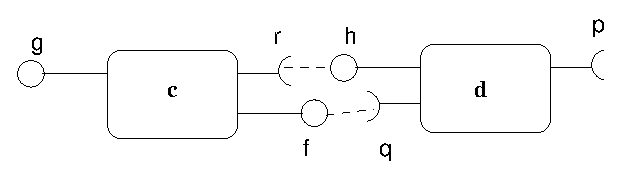
\epsfig{width=.4\textwidth,file=figures/fig-compo-contrex.eps}
    \caption{Contre-exemple}
    \label{fig-compo-contrex}
\end{figure}

On v\'erifie imm\'ediatement que $c$ et $d$ sont bien des composants
fiables pour leurs facettes et r\'eceptacles respectifs.
Le langage de $L_{\cal A}$,
selon la d\'efinition \ref{def:assemblages}, est :
$$
L_{\cal A} = h_X(\Tr(c)) \mix_{h_X(\ialph(c)),\ialph(X)} L_X
\mix_{\ialph(X),h_X(\ialph(d))} h_X(\Tr(d)),
$$
que l'on peut d\'evelopper en 
$$
\begin{array}{c}
((f\rightarrow mi() r\rightarrow mk() r\leftarrow mk() f\leftarrow
mi()) + (g\rightarrow mj() r\rightarrow mk() r\leftarrow mk() g\leftarrow
mj()))^*  \\
    \mix_{\ialph(c),\ialph(X)}   \\
((q\rightarrow mi() f\rightarrow mi())^* \sh (f\leftarrow mi() q\leftarrow
    mi())^* \sh  (r\rightarrow mk() h\rightarrow mk())^* \sh (h\leftarrow mk() r\leftarrow mk())^*) \\
\mix_{\ialph(X),\ialph(d)}   \\
(h\rightarrow mk() q\rightarrow mi() q\leftarrow mi() p\rightarrow
ml() p\leftarrow ml() h\leftarrow mk())^*.     
\end{array}
$$
Le langage r\'esultant est 
$$
f\rightarrow mi() + (g\rightarrow mj() r\rightarrow mk() h\rightarrow mk()),
$$
 et clairement
\begin{align*}
    \Pi_{h_X(\ialph(f))}(L_{\cal A}) \not\sim h_X(L_f) &\mbox{~et~} &\Pi_{h_X(\ialph(p))}(L_{\cal A}) \not\sim h_X(L_p),
\end{align*}
donc ${\cal A}$ n'est pas un composant fiable pour ses facettes et
r\'eceptacles.

Le cycle de d\'ependances entre les facettes et r\'eceptacles
connect\'es de $c$ et $d$ ne pose pas en soi de probl\`emes :  ce
qui pose probl\`eme ce sont les d\'ependances existant dans les
langages de $c$ et $d$ entre leurs facettes et  r\'eceptacles
connect\'es respectifs. Ce probl\`eme peut-\^etre lev\'e de deux
mani\`eres :
\begin{itemize}
  \item soit en s'assurant qu'il n'existe pas de mots dans le langage
  des composants assembl\'es induisant un ou plusieurs cycles de
  d\'ependances ;
\item soit en restreignant les op\'erations d'assemblage corrects
  \`a celles qui sont garanties ne pas introduire de cycles. 
\end{itemize}
Nous allons donc montrer que l'absence de cycle
est une condition suffisante pour obtenir un assemblage fiable. 

\subsubsection{Assemblage de deux composants}

Nous consid\'erons un assemblage form\'e de deux composants $c$ et
$d$ tel que les connexions de l'assemblage relient uniquement des
ports requis de $c$ \`a des ports fournis par $d$. Nous montrons
alors que si les deux composants sont fiables pour leurs ports
respectifs, alors l'assemblage r\'esultant est fiable pour les ports
non connect\'es. 

\begin{lemma}[Composition deux \`a deux]
\label{lem:assemblage-de-deux}
    Soit $c=\langle Port(c), \Tr(c) \rangle $ et $d=\langle Port(d),
    \Tr(d) \rangle $ deux instances de composants et $X$ un ensemble
    de connexions tels que :
    \begin{itemize}
      \item $\forall (e,p)\in elem(X)$, $e=c$ ou $e =d$ ;
      \item $\forall \chi \in X, \chi=(c,r,d,f)$ : les connexions
      ne concernent que des ports requis de $c$ avec des ports fournis
      de $d$.
    \end{itemize}
    Alors, si $c$ et $d$ sont \emph{fiables}, l'assemblage ${\cal A} = \langle
    \{c,d\},X\rangle$  est tel que : 
    \begin{enumerate}
      \item le langage de l'assemblage $L_{\cal A}$ est
        contractuellement fiable pour l'ensemble des ports $p$ de $Port(c)\cup Port(d) \setminus \{ p \mid (c,p) \in elem(X)\}$ ;
      \item pour toute facette $p=(f,I,\mathtt{facet})$ de $Port(c)\cup
        Port(d) \setminus \{ p \mid (c,p) \in elem(X)\}$, le langage
        $L_{\cal A}$ pr\'eserve l'ind\'ependance de la facette $p$.
    \end{enumerate}
\end{lemma}

La figure \ref{fig-compo-proof} est une repr\'esentation
sch\'ematis\'ee de l'assemblage $\cal A$ pour deux composants : les ports  des
des deux composants concern\'es qui ne sont pas  dans $X$ sont
repr\'esent\'es en traits pleins dans la partie droite et l'on verra
ult\'erieurement que l'on obtient ainsi un nouveau composant ou
composite. 

\begin{figure}[htbp]
    \centering
    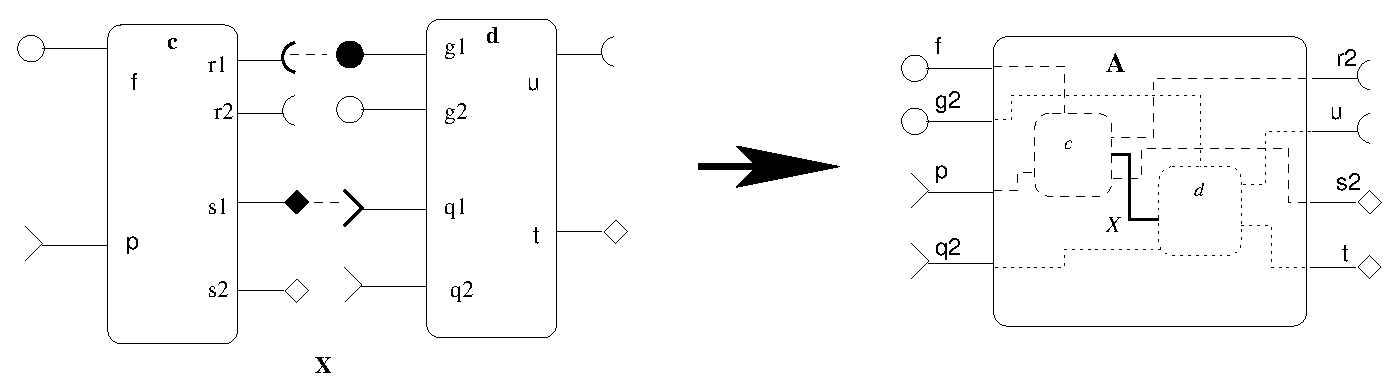
\epsfig{width=.8\textwidth,file=figures/fig-compo-proof.eps}
    \caption{Composition de $c$ et $d$}
    \label{fig-compo-proof}
\end{figure}

\begin{proof}[Composition]
    Nous montrons par induction que tout mot de $L_{\cal A}$ dont les
    pr\'efixes respectent les propri\'et\'es de fiabilit\'e contractuelle et
    d'ind\'ependance des facettes est lui-m\^eme un mot respectant
    ces propri\'et\'es. Autrement dit, si $u$ est un mot de $L_{\cal
    A}$ respectant ces propri\'et\'es, quelque soit la  mani\`ere de
    prolonger ce mot pour obtenir des mots de $L_{\cal A}$, on obtient
    des mots respectant les propri\'et\'es de fiabilit\'e
    contractuelle et d'ind\'ependance des facettes.

\textbf{Si $u=\epsilon$ :}

    Le mot vide $\epsilon$ appartient bien \`a $L_{\cal A}$ et
    trivialement, 
    $\epsilon$ respecte les contrats de chacun des ports de $\cal A$
    par d\'efinition de la propri\'et\'e de relation contractuelle.
    De m\^eme, l'ind\'ependance des facettes est \'evidemment respect\'ee.

\textbf{Si $u\neq\epsilon$ :}

Par hypoth\`ese d'induction :
\begin{itemize}
  \item pour tout port $p\in Port(\cal A)$, $\Pi_{\ialph(p)}(u) \in L_p$ ;
  \item pour toute facette $f\in Port({\cal A})$, l'ind\'ependance de $f$ est respect\'ee. Notons
    $F=\{(f,I,\mathtt{facet}) \in Port({\cal A})\}$ cet ensemble, l'on
    consid\'ere donc que  $u$ est de la forme $u=i_1 u_1o_1 i_2
    u_2 o_2 \dots   i_n u_n o_n$ avec :
    \begin{itemize}
      \item $i_1\in In(\ialph(f))$, $o_1\in Out(\ialph(f))$ pour un
        $f$ non connect\'e quelconque,
      \item et $u_i\in h_X(\ialph({\cal
          A}) \setminus \bigcup_{p\in F}ialph(p))^*$ ;
    \end{itemize}
  \item $u = v \mix x \mix w$
    avec $v \in h_X(\Tr(c))$, $w\in h_X(\Tr(d))$ et $x\in L_X$.
\end{itemize}

    Soit $a\in \ialph({\cal A})$  telle que $ua\in
    L_{\cal A}$. Si $a\in \ialph(p), p\in Port(c)\cup Port(d)\setminus
    Port({\cal A})$, $p$ un port connect\'e de l'assemblage, $ua$ est
    de toute \'evidence contractuellement correct pour les ports de
    $Port({\cal A})$ et il
    suffit donc de consid\'erer les diff\'erentes possibilit\'es de prolonger le
    mot $u$ par une lettre $a\in \ialph(p)$ pour $p\in Port({\cal A})$
    un port non connect\'e de l'assemblage :
    \begin{enumerate}
      \item si $a\in \ialph(p), p\in \Rc(d)\cup \Source(d)\cup \Sink(d)$, par hypoth\'ese de
        fiabilit\'e de $d$, $wa$ est fiable pour $p$ et donc 
        $$
        u'=ua = v\mix x \mix wa
        $$
        est fiable et respecte l'ind\'ependance des facettes ;
      \item si $a\in \ialph(p), p\in \Rc(c)\cup \Source(c)\cup \Sink(c)$, par hypoth\'ese de
        fiabilit\'e de $c$, $va$ est fiable pour $p$ et donc 
        $$
        u'=ua = va\mix x \mix w
        $$
        est fiable et respecte l'ind\'ependance des facettes ;
      \item si $a\in \ialph(f), f\in \Fc(d)$, par hypoth\'ese de
        fiabilit\'e de $d$, $\Pi_{\ialph(f)}(w)i \in \Tr(f) \implies wi \in \Tr(d)$ et il existe $o\in h_c(Out(\ialph(f)))$ tel que
        $wiyo\in \Tr(d)$. Par hypoth\`ese d'ind\'ependance des facettes
        de $d$, $y\in \ialph(d)\setminus
        \cup_{p\in \Fc(d)\cup \Sink(d)}ialph(p))^*$. On a donc  
        $$
        u'= uiyo = v\mix x \mix wiyo
        $$
        est fiable et respecte l'ind\'ependance des facettes de ${\cal A}$.
    \end{enumerate}

    Nous d\'etaillons manintenant le cas o\`u $a$ est une lettre
    d'une facette de $c$.
    Soit $f$ une facette de $c$ et $i\in h_c(In(\ialph(f)))$ tel que
    $ui\in L_{\cal A}$. Par hypoth\`ese de fiabilit\'e de $c$,
    $\Pi_{\ialph(f)}(v)i \in \Tr(f) \implies vi \in \Tr(c)$ et il existe $o\in h_c(Out(\ialph(f)))$ tel que
    $viyo\in \Tr(c)$, avec $y\in h_X(\ialph(c)\setminus
    \cup_{p\in \Fc(c)\cup \Sink(c)}ialph(p))^*$. 
    
    Si $y=\epsilon$, alors 
    $$
    (v \mix x \mix w)io = (vio \mix x \mix w) \subseteq L_{\cal A},
    $$
    donc $L_{\cal A} \sim f$ et trivialement ${\cal A}\perp f$. 
    
    Si $y\neq\epsilon$, alors par hypoth\`ese d'ind\'ependance des
    facettes de $c$, $y\in (\cup_{p\in\Rc(c)\cup
      \Source(c)}\ialph(p))^*$ et par hypoth\`ese de fiabilit\'e de
    $c$ on a
    $$
    y \in (o_1 i_1) \sh (o_2 i_2) \sh \dots \sh (o_n i_n),
    $$ 
    avec 
    \begin{eqnarray}
        o_j \in \ialph(r), \mbox{~pour~} r\in \Rc(c) \implies
        \Pi_{\ialph(r)} (v o_j i_j) \in \Tr(r) \label{eq:c-fiab-rec-ncnx}\\
        \mbox{~et~} \notag\\
        o_j \in \ialph(s), \mbox{~pour~} s\in \Source(c) \implies
        i_j = \epsilon \mbox{~et~} \Pi_{\ialph(s)} (v o_j ) \in
        \Tr(s).\label{eq:c-fiab-puits}
\end{eqnarray}
$y$ est constitu\'e uniquement de messages arbitrairement
    entrelac\'es en fonction du langage de $c$ concernant des
    r\'eceptacles et puits de $c$. 

Soit $I\subseteq \mathbb{N}$ un ensemble d'indices $I$, $I$ est
totalement ordonn\'e par la relation d'ordre naturelle des entiers et
l'on \'ecrira 
$$
\bigodot_{i\in I} u_i
$$
la concat\'enation d'un ensemble de mots indic\'es par des
\'el\'ements de $I$ dans l'ordre induit par cet ensemble : 
$$
\bigodot_{i\in I} u_i = \bigodot_{j=1}^{\vert I\vert} u_{i_j} = u_{i_1} u_{i_2} \dots u_{i_n},  
$$
avec pour tout $i_j,i_k$, $j<k \Leftrightarrow i_j < i_k$.


    Soit $I\subseteq \{1,\dots,n\}$ un \emph{marquage} tel que $\forall j \in I, \exists
    (c,r,d,g)\in X$ tel que $o_j$ et 
    $i_j$ appartiennent \`a $\ialph(r)$, 
    \begin{align*}
        y_d&=\Pi_{\cup_{\ialph(g), (c,r,d,g)\in X}}(y)\\
        &=\bigodot_{j\in I} o_j i_j.
    \end{align*}
    
    Comme $c \sim r$, $d\sim g$ et $d \perp g, \forall g \in \Fc(d)$
    tels que $(c,r,d,g)\in X$, alors pour tout $j\in I$ il existe $z_j$ tel que 
    $$
    w \bigodot_{j\in I} (i_{g_j} z_j o_{g_j}) \in \Tr(d)
    $$ 
    avec $z_j \in h_X(\ialph(d)\setminus \cup_{p\in \Fc(d)\cup
    \Sink(d)}\ialph(p))^*$ et $\Pi_{\ialph(g)}(w i_g o_g) \in \Tr(g),
    \forall g \Fc(d)$. Notons que l'inclusion de la projection dans le
    langage d\'ecoule du fait que $c\sim r$ et que $L_r=
    \bar{h}(L_g)$ donc les sorties produites par $L_c$ sur $r$ sont
    incluses dans l'ensemble de sorties produites par $L_r$, ce qui
    par application de $\bar{h}$ implique que les entr\'ees sur $d$
    par $g$  depuis $r$  sont incluses dans les entr\'ees possibles sur
    $L_g$.
    
    Pour tout $\chi =(c,r,d,g)$, par construction de $L_\chi$, pour
    tout $j\in I$, $x o_j i_{g_j}  o_{g_j} i_j \in L_\chi$ avec
    $i_{g_j}= \bar{h}(o_r),o_{g_j}=\bar{i}_j$. 

    Par ind\'ependance des facettes de $d$, on a
    \begin{align*}
        u' &= (viyo \mix x(\sh_{\{(r,g) \mid (c,r,d,g) \in
          X,\Pi_{\ialph(r)}(y)\neq \epsilon\}} o_r i_g o_g i_r) \mix
        w() \\
        &=(v \mix x  \mix w)i o_1 i_{g_1} z_1 o_{g_1} i_1 . o_2 i_{g_2} z_2
        o_{g_2} i_2  \dots o_k i_{g_k} z_k
        o_{g_k} i_k o.
    \end{align*}
    Comme $\forall i \in \ialph(f), \Pi_{\ialph(f)}(u')i \in L_{\cal
      A}$  et $\Pi_{\ialph(f)}(u')io \in \Tr(f)$, donc  
    $$
    \forall f\in \Fc(c), u' \sim f.
    $$ 
  
  Par hypoth\`ese de fiabilit\'e de $d$, on a bien $\forall j\in I$
  tel que $z_j\neq \epsilon$, pour tout r\'eceptacle et puits $q$
  de $d$, $\Pi_{\ialph(q)}(L_d) \geq L_q$ d'o\`u $\Pi_{\ialph(q)}(w
  z_j) \in L_q$, $\Pi_{\ialph(q)}(u z_j) \in L_q$,  donc  
  $$
  \forall q\in \Rc(d)\cup \Sink(d), u' \sim q.
  $$  
  
  Enfin, en appliquant une construction similaire pour toutes les
  sources de $c$, on d\'eduit 
  $$
  \forall s\in \Source(d)\setminus elem(X), u\sim s \implies u' \sim s.
  $$  

  De m\^eme, pour toutes les facettes non connect\'ees de $d$, par
  hypoth\`ese d'ind\'ependance et de fiabilit\'e, on a 
  $$
  \forall f\in (\Fc(d)\cup \Source(d))\setminus elem(X), u' \sim f.
  $$  

  De \eqref{eq:c-fiab-rec-ncnx} et \eqref{eq:c-fiab-puits} on d\'eduit 
  \begin{align*}
      \forall r\in \Rc(c)\setminus elem(X), u'\sim c&\mbox{~et~}& \forall r\in
      \Sink(c)\setminus elem(X), u'\sim c.
  \end{align*}

  Enfin, en appliquant une construction similaire pour toutes les
  sources de $c$, on d\'eduit 
  $$
  \forall s\in \Source(d)\setminus elem(X), u\sim s \implies u' \sim s.
  $$  
  
  On a donc, pour tout les ports $p$ non connect\'es  de $c$ et $d$,
  $u'\sim p$ donc ${\cal A}$ est fiable pour $Port({\cal A})$ et
  respecte l'ind\'ependance des facettes de $Port({\cal A})$.\hfill\qed
\end{proof}

\subsubsection{Composite}

Pour pouvoir \'etendre ce r\'esultat de mani\`ere inductive d'un assemblage de deux
composants \`a un assemblage de $n$ composants, il est n\'ecessaire
de pouvoir construire un composant \`a partir d'un assemblage. Nous
d\'efinissons donc dans cette section la notion de \emph{composite},
c'est \`a dire de composant form\'e \`a partir d'un assemblage.
Pour ce faire, il faut fournir au nouveau composant 
une identit\'e propre et  veiller \`a ce que les ports non
connect\'es soient correctement renomm\'es, afin d'\'eviter des
collisions de noms avec des ports de m\^eme noms fournis par d'autres
composants participant du m\^eme assemblage.
On obtient ainsi une entit\'e autonome et opaque qui se comporte
comme n'importe quel autre composant. 

\begin{definition}[Composite]
\label{def:composite}
\'Etant donn\'e un assemblage ${\cal A} = \langle B,X\rangle$
\emph{fiable} pour l'ensemble de ses ports non connect\'es
$Port({\cal A})$, on
d\'efinit l'instance de composant $c=\langle P, L_c\rangle$ comme
suit :
\begin{itemize}
  \item $P = \cup_{c_i\in B} \{(c_i^p,T,g)\mid (p,T,g) \in Port({\cal A})\}$ est l'ensemble des ports de $c$ ;
\item $L_c = h_c(L_{\cal A})$ est le langage de $c$ ;
\end{itemize}
avec le morphisme $h_c$ d\'efini comme :
$$\begin{array}{rlcl}
h_c:&\ialph({\cal A}) &\longrightarrow& \ialph(c) \\
&(c_i,p,\gamma_2,\varrho_2,k,m,\vec{x},v)&\longmapsto&(c,c_i^p,\gamma_2,\varrho_2,k,m,\vec{x},v)
\mbox{~si~} (c_i,p) \not\in elem(X)\\
&(\gamma_1,\varrho_1,c_i,p,k,m,\vec{x},v)&\longmapsto&(\gamma_1,\varrho_1,c,c_i^p,k,m,\vec{x},v)
\mbox{~si~} (c_i,p) \not\in elem(X)\\
&x&\longmapsto&\epsilon\mbox{~sinon.}
\end{array}$$
\end{definition}

Classiquement, l'op\'eration d'encapsulation que repr\'esente la
formation d'un composite \`a partir d'un assemblage a pour effet de
supprimer du langage de ce dernier les messages relatifs aux ports
connect\'es. Les ports restant, non connect\'es, sont alors
renomm\'es et l'on obtient une nouvelle instance de composants
d'identit\'e $c$.

\subsubsection{Assemblage fiable}

Une derni\`ere condition pour \'etendre la composition de deux
composants \`a $n$ composants assembl\'es sur un ensemble de
connexions est li\'ee \`a la \emph{topologie } des connexions. 
Pour tout ensemble de connexions $X$, on peut d\'efinir un graphe dirig\'e
$G_X=(S,A)$ o\`u $S$ est l'ensemble des sommets du graphe et $A\subseteq
S\times{}S$ est l'ensemble des arcs du graphe, construit comme suit :
\begin{itemize}
  \item $S = elem(X)$ ;
  \item $A = \{ ((c,p),(c,p')) \mid p\in \Fc(c)\cup\Sink(c)\wedge
  p'\in \Rc(c) \cup \Source(c)\} \cup \{ ((c,p),(c',p')) \mid
  (c,p,c'p')\in X\}$.
\end{itemize}

\begin{definition}[Enesmble de connexions consistant]
\label{def:cnx-consistantes}
Soit $X$ un ensemble de connexions, $X$ est \emph{consistant} si et
seulement si le graphe de connexion induit par $X$, $G_X$, est acyclique.
\end{definition}

\begin{theoreme}[Compositionnalit\'e]
\label{th:compositionnalite}
    Soit ${\cal A} = \langle B,X \rangle$ un assemblage tel que
    l'ensemble $X$ des connexions est \emph{consistant} (d\'efinition
    \ref{def:cnx-consistantes}) et tel que tout composant $c\in B$ est
    \emph{fiable} (d\'efinition \ref{def:fiab-dun-comp}),
    alors ${\cal A}$ est \emph{fiable} pour l'ensemble des ports non
    connect\'es $Prot({\cal A})$.
\end{theoreme}

\begin{proof}
    Le graphe $G_X=(S,A)$ induit par l'ensemble de connexions $X$
    (d\'efinition \ref{def:cnx-consistantes}) \'etant dirig\'e
    acyclique, on peut \'enum\'erer $elem(X)$, l'ensemble des
    sommets de $G_X$, suivant un tri topologique associ\'e \`a
    l'ordre partiel induit par les arcs de $G_X$. D'o\`u 
    $$
    \forall s,s' \in S, s\leq s' \Leftrightarrow 
    \begin{array}{l}
s = s' \\
\mbox{ou~} (s,s')\in A \\
\mbox{ou~} \exists s''\in S, s\leq s'' \mbox{~et~} s''\leq s'.
    \end{array}
    $$
    
    En particulier, si $(c,r,d,f)\in X$, $(c,r)\leq (d,f)$  et par
    acyclicit\'e du graphe, il n'existe pas de ports $p$ dans
    $Port(c)$,$q$ dans $Port(d)$ tels que  $(d,q)\leq (c,p)$. 
    Soit $n=\vert B\vert$, alors l'ordre
    d\'efini ci-dessus induit une \emph{bijection} $\iota:B
    \rightarrow \{1,\dots,n\}B$ qui associe un indice \`a chaque composant. On a
    donc $\iota(c)=\iota(d) \implies c= d$ et 
    $$
    \iota(c)< \iota(d) \implies 
    \forall (c,p,d,q)\in X, p\in \Rc(c)\cup \Source(c) \mbox{~et~} q\in
    \Fc(d)\cup \Sink(d).
    $$

    Par induction sur l'ordre de $\iota$ :
    \begin{itemize}
      \item pour $c$ tel que $\iota(c) = 1$, par hypoth\`ese $c$ est
        fiable et donc ${\cal
          A} = \langle \{c\},\emptyset \rangle$ est fiable ;
      \item soit $k\in \{1,\dots n\}$, on suppose que le composite  ${\cal C}_k$
      produit \`a partir de l'assemblage ${\cal A}_k$  tel que ${\cal A}_k = \langle
      \{\iota^{-1}(1),\dots,\iota^{-1}(k) \}, X_k=\{(c,p,d,q)\mid \iota(c)\leq k
      \mbox{~et~} \iota(d)\leq k\}\rangle$ est fiable. Soit ${\cal
      A}_{k+1}$ l'assemblage d\'efini par ${\cal A}_{k+1} = \langle
      \{{\cal C}_k,\iota^{-1}(k+1)\}, X_{k+1}=\{(c,p,d,q)\in X
      \mid d=\iota^{-1}(k+1)\}\rangle$ :
      \begin{itemize}
        \item si $X_{k+1} = \emptyset$, alors ${\cal A}_{k+1}$ est
        l'union sans connexion de deux composants fiables et par
        cons\'equent est fiable,
      \item sinon, par application du lemme
        \ref{lem:assemblage-de-deux} avec $c={\cal C}_k$ et
        $d=\iota^{-1}(k+1)$, on a bien ${\cal A}_{k+1}$ est fiable ce qui
        termine l'induction.\hfill\qed
      \end{itemize}
    \end{itemize}
\end{proof}

\subsection{Composition \& Mod\`eles}

Nous avons dans les pr\'ec\'edentes sections d\'efini la
composition en termes d'\emph{instances de composants}. On peut tout
aussi bien consid\'erer qu'il est int\'eressant de sp\'ecifier
directement un assemblage. Pour ce faire, nous \'etendons la syntaxe
et la s\'emantique du langage \textsf{FIDL} (voir chapitre
\ref{chap-fidl}). 

La syntaxe --- au niveau \textsf{IDL3} du langage --- de la
d\'efinition d'un \emph{composite}  est d\'ecrite 
par la grammaire dans la figure \ref{fig-syn-fidl-assm}. Elle
introduit un mot-cl\'e $\mathtt{assembly}$  et permet
de d\'ecrire le composite correspondant en nommant les composants qui
le r\'ealisent et en d\'efinissant les connexions entre ces
composants. 
Les lex\`emes $\mathtt{id}$ et $\mathtt{fqname}$ d\'esignent
respectivement un identifiant valide en \textsf{IDL3} et un nom
qualifi\'e.

\begin{figure}
    \begin{equation}
        \label{eq:syn-fidl-assm}\begin{array}{r@{\quad\rightarrow\quad}l}
            Composite & \mathtt{assembly}\ \mathsf{id}\ \mathtt{\{}\
              Assembly\ \mathtt{\} ;} \\
            Assembly & Assembly\ Component \mid Assembly\ Connection 
            \mid Assembly\ Hide\mid \epsilon \\
            Component & \mathtt{component}\ Type\ \mathsf{id}\ \mathtt{;}  \\
            Connection & \mathtt{connection}\ Port\ Port\ \mathtt{;}  \\
            Hide & \mathtt{hide}\ Port\ \mathtt{;}  \\
            Port & \mathsf{id}.\mathsf{id} \\
            Type & \mathtt{fqname}
        \end{array}
    \end{equation}
    \caption{Syntaxe des composites}
    \label{fig-syn-fidl-assm}
\end{figure}

Cette syntaxe permet de d\'efinir un nouveau --- type de ---
composant par assemblage de composants plus primitifs. Les
d\'efinitions relatives aux assemblages (d\'efinition
\ref{def:assemblages}) et aux composites (d\'efinition \ref{def:composite}) doivent
\^etre simplement adapt\'ees : le terme instance de composant
d\'esigne alors simplement un composant nomm\'e de l'assemblage. Les
d\'efinitions de langages et d'alphabets sont identiques. La seule
modification importante concerne le \emph{masquage} de ports ce qui
implique de red\'efinir l'ensemble des ports d'un composite.

\begin{definition}[Masquage de ports]
Soit $C$ un composant et $H\subseteq \Fc(C)\cup \Sink(C)$  un ensemble de ports
\emph{masqu\'es}, alors on d\'efinit le composant $C'=\langle Port(C)
\setminus H,\Tr(C) \rangle$.
\end{definition}

On notera que le langage de $C'$ est identique au langage de $C$. La
suppression des ports masqu\'es  de l'ensemble de ports implique
n\'ecessairement l'impossibilit\'e de se connecter sur les ports
masqu\'es donc l'impossibilit\'e de \og produire \fg{} les mots
induits par un appel ou un message sur une facette ou un puits
masqu\'e. Par ind\'ependance des facettes, on est assur\'e
toutefois de conserver un comportement fiable du composant dont les
ports sont masqu\'es. 

%% \begin{definition}[Composite (2)]
%% \label{def:type-composite}
%%     Un \emph{composite} $\cal C$ est d\'efini par :
%%     \begin{itemize}
%%       \item un ensemble $B$ de couples $(C,n)$ o\`u $C$ identifie un
%%         composant et $n$ est un nom \emph{unique} dans $B$ ;
%%       \item un ensemble de connexions $X$ constitu\'e de quadruplets
%%         $(c,r,d,f)$ o\`u $c,d$ sont des noms d'\'el\'ements de $B$ et
%%         $r$ --- resp. $f$ ---  un  noms de port appartenant respectivement au composant
%%         identifi\'e par $c$ --- resp. $d$.
%%     \end{itemize}
%%     Le langage de l'assemblage $L_{\cal C}$ et son alphabet sont d\'efinis par :
%%     \begin{eqnarray}
%%         \ialph({\cal C}) = \bigcup_{(C,n)\in B}h_X(h_n(\ialph(C))),\label{eq:alph-assemblage} \\
%%         L_{\cal C} = (\bigsh_{(C,n)\in B} h_X(h_n(L_C)))\bigmix_{\ialph({\cal
%%             C}),\ialph(X)} (\bigsh_{\chi \in X} L_\chi). \label{eq:lang-assembly}
%%     \end{eqnarray}
%%     Le morphisme $h_n$ pour un nom de composant $n$ est d\'efini
%%     simplement par 
%%     $$
%%     \begin{array}{rlcl}
%%         h_n:&\ialph({\cal C}) &\longrightarrow& {\cal E} \\
%%         &(\gamma,p,\gamma_2,\varrho_2,k,m,\vec{x},v)&\longmapsto&(n,p,\gamma_2,\varrho_2,k,m,\vec{x},v)\\
%%         &(\gamma_1,\varrho_1,\gamma,p,k,m,\vec{x},v)&\longmapsto&(\gamma_1,\varrho_1,n,p,k,m,\vec{x},v)\\
%%     \end{array}
%%     $$
%% Un composite $\cal C$ est un composant $\langle Port({\cal C}),
%% L_{\cal C}\rangle$ o\`u 
%% $$
%% Port({\cal C}) = \{h_{p}^{C_n}((p,T,g)) \mid (
%% $$
%% \end{definition}


\subsection{V\'erification}
\label{sec:verification}
Dans la section \ref{sec:compositionnalite}, nous avons d\'efini des
propri\'et\'es attendues des composants --- ind\'ependance des
facettes, respect des contrats des ports --- et des assemblages ---
acyclicit\'e du graphe de connexion --- nous permettant de produire
\emph{par construction} des \emph{composites} poss\'edant ces
propri\'et\'es sans qu'il soit n\'ecessaire de red\'emontrer
leur existence. On a ainsi montr\'e que le mod\`ele \textsf{FIDL}
\'etait r\'eellement \emph{compositionnel} pour certaines
propri\'et\'es fondamentales. 

Il reste bien s\^ur \`a v\'erifier que les composants atomiques
utilis\'es dans un assemblage poss\`edent effectivement ces
propri\'et\'es. Dans le cas d'instances concr\`etes de composants,
ce probl\`eme sera \'etudi\'e au chapitre \ref{cha:test}
consacr\'e au test de composants \textsf{FIDL}. Dans le cas 
de \emph{sp\'ecifications} de composants --- simplement appel\'es
\emph{composants}, cette v\'erification doit \^etre r\'ealis\'ee
\`a partir de la sp\'ecification du comportement du composant.

Cette v\'erification rel\`eve \emph{a priori} des techniques de
\emph{v\'erification de mod\`eles} --- \emph{model-checking} en
anglais --- qui constituent un champs de recherche particuli\`erement
actif. Ceci ne rel\`eve toutefois pas du c\oe ur du sujet de cette
th\`ese et nous nous contentons dans cette section d'equisser une
strat\'egie permettant de construire un probl\`eme de model-checking
\`a partir d'un mod\`ele \emph{FIDL} de composant pour v\'erifier
les deux propri\'et\'es n\'ecessaires \`a la compositionnalit\'e
des composants :
\begin{itemize}
  \item l'ind\'ependance des facettes ;
  \item le respect des contrats li\'es aux diff\'erents ports.
\end{itemize}

\subsubsection{Ind\'ependance des facettes}

Le probl\`eme de l'ind\'ependance des facettes est
plus simple que celui du respect des ports. En
effet, on peut transformer la propri\'et\'e
\ref{def:indep-des-facett-1}  d'ind\'ependance sous la forme de l'\'equation
\eqref{eq:prop-independance} : pour toute s\'equence $u$ de messages abstraits
--- voir \'equation \eqref{eq:def-morph-abst} --- du langage du
composant, la projection sur l'union des alphabets abstraits des
facettes et puits du
composant du langage r\'esiduel de $u$ est \'egale au
produit de m\'elange de la projection du langage r\'esiduel de $u$
sur l'alphabet abstrait de chacune de ses facettes 
et puits. 

\begin{prop}
Soit $C=\langle Port(C),\Tr(C) \rangle$ un composant et soit
$\Lambda_C=h_\lambda(\Tr(C))$ le langage associ\'e \`a $C$ sur l'\emph{alphabet
abstrait} des messages. Alors,  $ \forall f \in \Fc(C),C\perp f,$ si et seulement si
\begin{equation}
    \begin{array}{c}
        \forall u \in \Lambda_C, \\
        \prod_{\bigcup_{p\in \Fc(C)\cup \Sink(C)}h_\lambda(\ialph(p))}(u^{-1}\Lambda_C) =
        \bigsh_{p \in \Fc(C) \cup \Sink(C)} \Pi_{h_\lambda(\ialph(p))}(u^{-1}\Lambda_C).
    \end{array}\label{eq:prop-independance}
\end{equation}
\end{prop}
Autrement dit, pour chaque facette et puits du composant, il existe
toujours dans le langage du composant une s\'equence de messages
o\`u n'intervient aucun autre facette ou puits du composant. 

Cette formulation nous permet de travailler pour la v\'erification de cette
propri\'et\'e non pas sur le langage de l'expression de $C$ avec les contraintes sur le contenu des
messages mais uniquement sur les  \emph{enveloppes} des
messages, donc sur un langage reconnaissable par un automate
standard avec un alphabet fini. 

Pour chaque \'etat $q$ d'un automate, le langage associ\'e \`a $q$,
$L_q$, est pr\'ecis\'ement le langage r\'esiduel de $L$ ou quotient
\`a gauche  de $L$ pour tous les mots $u$ tels qu'il existe un chemin
dans l'automate entre $q_0$ et $q$. Il suffit donc de v\'erifier cette
propri\'et\'e pour chaque \'etat $q$ de l'automate associ\'e \`a $\Lambda_C$. 

\subsubsection{Respect des ports}

La v\'erification du respect des ports, et en particulier du respect
des contrats des facettes et r\'eceptacles --- propri\'et\'es
\ref{def:respect-receptacles} et \ref{def:respect-facettes} --- est
nettement plus ardue puisque dans ce cas, il est n\'ecessaire de
prendre en compte les valeurs, contraintes et  fonctions
n\'ecessaires \`a la construction du corps des messages. 
De toute \'evidence, sans hypoth\`ese suppl\'ementaire sur ces \'el\'ements, cette v\'erification est
impossible. 

Un certain nombre de techniques existent pour le \emph{model-checking} de
programmes concurrents, y compris avec des variables. L'approche
introduite dans \cite{smv-thesis} et qui est \`a la base de l'outil
\textsf{SMV} est une des plus connue. Cette approche permet de
g\'erer le probl\`eme de l'explosion du nombre d'\'etats dans
l'analyse d'accessibilit\'e d'un graphe par
l'abstraction d'ensembles d'\'etats sous forme de \emph{Diagrammes de D\'ecision
Binaires}. Une autre approche plus r\'ecente et prometteuse, bas\'ee
sur la \emph{s\'emantique de jeu}, est propos\'ee dans
\cite{abramsky-etal} et d\'etaill\'ee dans \cite{ghica-tg}. Dans une
s\'emantique de jeu\cite{algo-game-sem}, l'ex\'ecution d'un
programme est mod\'elis\'ee comme un \emph{jeu \`a 2 joueurs} entre le
programme et  son environnement. Le principal int\'er\^et de cette
approche est sa compositionnalit\'e qui permet d'interpr\'eter des
fragments de langage comme des \emph{strat\'egies} et de construire une s\'emantique par la
composition des interpr\'etations de ces fragments. Un autre
int\'er\^et est qu'une strat\'egie est d\'efinie comme un langage
rationnel. De notre point de vue, l'utilisation de cette s\'emantique
pr\'esenterait l'int\'er\^et d'unifier dans un m\^eme cadre ---
celui des langages rationnels --- les diff\'erentes parties du
langage \textsf{FIDL}. 

Dans un certain nombre de cas simples, par exemple lorsque les
donn\'ees sont contraintes par des pr\'edicats de base, en l'absence de
fonctions auxiliaires complexes et/ou avec des types de donn\'ees finis, la
v\'erification peut-\^etre faite directement par projection vers un
\emph{model-checker}. 

Le mod\`ele \textsf{FIDL} \'etant bas\'e sur des \emph{automates finis avec
  variables}, on peut  raisonnablement supposer qu'il est
possible d'utiliser les techniques esquiss\'ees ci-dessus pour
  v\'erifier des propri\'et\'es d'un mod\`ele \textsf{FIDL}.

\section{H\'eritage}

\label{sec:heritage-comportemental}
Dans le langage \textsf{FIDL}, les interfaces repr\'esentent des contrats
propos\'es par des composants au travers de facettes et utilis\'es par
ceux-ci au travers de r\'eceptacles. Au niveau purement syntaxique de
l'\textsf{IDL3}, les probl\`emes pos\'es par l'h\'eritage sont extr\^emement r\'eduits,
d'autant plus que le langage n'autorise pas la surcharge de m\'ethodes.
Une interface h\'eritant d'une ou plusieurs autres interfaces \emph{importe}
simplement des m\'ethodes --- signatures --- des super-interfaces et offre une garantie
minimale au client. 

Lorsqu'on s'int\'eresse aux interfaces en tant que sp\'ecification
comportementale des communications entre deux composants au travers de
ports identifi\'es, l'h\'eritage pose divers probl\`emes :
\begin{itemize}
  \item peut-on dans une sous-interface red\'efinir le comportement
    d'une m\'ethode, c'est-\`a-dire changer le contenu des param\`etres attendus en entr\'ee et
    retourn\'es en sortie par la m\'ethode --- bien entendu sans changer
    leur type ?
  \item peut-on \'etendre le comportement d'une super-interface avec
    d'autres m\'ethodes et de quelle mani\`ere ?
  \item peut-on restreindre le comportement d'une super-interface,
    c'est-\`a-dire la sp\'ecialiser et de quelle mani\`ere ?
  \item que se passe-t'il lorsqu'une interface h\'erite de plusieurs
    interfaces d\'efinissant les m\^emes m\'ethodes --- signature identique
    --- mais avec des comportements diff\'erents ?
  \item comment est d\'efini --- et calcul\'e --- l'ensemble de traces
    d'une sous-interface par rapport \`a ses super-interfaces et, corollaire, que
    doit-on r\'e\'ecrire et que peut-on r\'eutiliser ?
\end{itemize}

La relation de sous-typage la plus commun\'ement utilis\'ee
dans le domaine des langages orient\'es objets 
est la notion de \emph{sous-typage comportementale} introduite dans
\cite{liskov94behavioral} et qui s'\'enonce comme suit (traduction
par nos soins) :
\begin{definition}[Sous-typage Comportemental]
Si $\phi(x)$ est une propri\'et\'e prouvable pour tous les  objets $x$ de
type $T$, alors $\phi(y)$ doit \^etre vraie pour tous les objets  $y$ de type
$S$ o\`u  $S$ est un sous-type de $T$.
\end{definition}
Dans le contexte de \cite{liskov94behavioral}, les propri\'et\'es
auxquelles on s'int\'eresse sont des propri\'et\'es de
\emph{s\^uret\'e} : invariants sur l'\'etat (observable) des objets
d'un type et comportement (propri\'et\'es sur l'historique), les
sp\'ecifications \'etant exprim\'ees sous la forme d'assertions
logiques (invariants de type, pr\'e- et post-conditions sur les m\'ethodes).
Ceci revient \`a dire que l'on peut toujours substituer un $y$ pour un
$x$ sans remettre en cause le fonctionnement des \emph{clients} de $x$. 

\subsection{Relation de sous-typage}

On va chercher \`a d\'efinir dans le cadre de sp\'ecifications
\textsf{FIDL} une notion de sous-typage
qui pr\'eserve les propri\'et\'es de compositionnalit\'e des
composants et donc la relation contractuelle existant entre un
fournisseur et un utilisateur d'une interface donn\'ee : pour tout
r\'eceptacle $r$ de type $I$, on doit pouvoir d\'efinir une
connection avec une facette $f$ de type $I$ ou d'un sous-type de (une
interface descendante de) $I$.

Pour ce faire, on va naturellement utiliser la \emph{relation
  contractuelle}  d\'efinie pr\'ec\'edemment (voir d\'efinition
  \ref{def:rel-contrat}). 

\begin{definition}[Sous-typage comportemental]
Soit deux  interfaces $I=\langle meth(I),\Tr(I)\rangle$ et $J=\langle
meth(J),\Tr(J)\rangle$, 
$J$ est un sous-type comportemental de $I$, ce qui est not\'e $I
\sqsubseteq J$ si et seulement si :
\begin{enumerate}
  \item $\ialph(I)\subseteq \ialph(J)$ ;
  \item et $\Tr(I) \lesssim \Tr(J).$
\end{enumerate}
\end{definition} 

Autrement dit, une sous-interface acceptera au moins toutes les
entr\'ees de sa super-interface et produira au plus toute les sorties
qu'aurait produite celle-ci, ce qui correspond aux propri\'et\'es usuelles
d'affaiblissement des pr\'econditions et de renforcement des post-conditions. 
Cette d\'efinition autorise une sous-interface \`a
red\'efinir le comportement de sa super-interface tant que la
transparence est respect\'ee pour les clients de la super-interface

\subsubsection{Types de donn\'ees}

La relation de sous-typage comportemental s'\'etend
naturellement aux types des param\`etres des messages et des valeurs
de retours. Il est alors n\'ecessaire de respecter la contravariance pour
les param\`etres en mode \textbf{in} et la covariance pour les
param\`etres en mode \textbf{out} et les valeurs de retours. Les
param\`etres en mode \textbf{in-out} ne peuvent donc varier. 

Nous supposons l'existence d'une relation de sous-typage sur
l'ensemble des donn\'ees ${\cal D}$ qui peut \^etre simplement la
relation d'inclusion des ensembles en consid\'erant que les types
sont des parties de ${\cal D}$. Pour tout couple de  types $T$ et $S$, $S$ est un
\emph{sous-type} de $T$ si et seulement si ${\cal D}_T\subseteq {\cal D}_S$. 

Soit deux interfaces $I$ et $J$ telles que $J$ est un sous-type de
$I$, et deux m\'ethodes $m_1=T\ m(T_1,\dots,
T_n) \in meth(I)$, $m_2=T'\ m'(T'_1,\dots, T'_n) \in
meth(J)$. Alors, $m_2$ est une
\emph{red\'efinition} valide de $m_1$ pour  la relation de
sous-typage si $m'=m$ et si :
\begin{itemize}
  \item les types des param\`etres en mode \textbf{in} sont plus
  \og larges \fg{} dans $m_2$ : 
$$
\forall T_i, i\leq in(m_1), {\cal D}_{T_i} \subseteq {\cal D}_{T'_i} ;
$$
\item les types des param\`etres en mode \textbf{out} sont plus
  \og larges \fg{} dans $m_1$ : 
$$
\forall T_i, i\geq out(m_1), {\cal D}_{T'_i} \subseteq {\cal D}_{T_i}.
$$

\end{itemize}
Notons que le langage \textsf{IDL} interdit la \emph{surcharge} des
m\'ethodes, c'est \`a dire l'utilisation d'un m\^eme nom pur deux
m\'ethodes diff\'erentes.

\subsubsection{Exceptions}

L'ensemble des exceptions susceptibles d'\^etre lev\'ees par une
m\'ethode $m$ est not\'e $exceptions(m)$. Les messages d'exception
constituent une classe diff\'erentes des appels et des retours de
m\'ethode, mais qui est prise en compte dans le langage de
l'interface. Un appel de m\'ethode et un retour d'exception sont
autoris\'es par les r\`egles de formation des langages d'interfaces
(voir la d\'efinition \ref{def:traces-interfaces}). 

Par cons\'equent, pour deux interfaces $I$ et $J$ avec $I\sqsubset J$
et deux m\'ethodes $m \in meth(I)$, $m'\in meth(J)$, $m'$ est une
red\'efinition valide de $m$ pour la relation de sous-typage si
$exceptions(m') \subseteq exceptions(m)$ : une m\'ethode peut choisir
de lever moins d'exceptions.

\subsection{Sous-typage \& Connexions}

Le principal int\'er\^et de pouvoir d\'efinir une relation de
sous-typage est bien entendu que cette relation s'int\`egre
harmonieusement dans les m\'ecanismes de connexion et de composition
du langage. 
Nous modifions donc la d\'efinition \ref{def:connexions} d'une connexion pour
autoriser la mise en relation de ports dont les types
respectifs appartiennent \`a une relation de sous-typage
comportemental. 

\begin{definition}[Connexion]
Une connexion $\chi$ entre deux ports $(p,I,g)$ et $(p',J,g')$ appartenant respectivement
\`a deux instances de composants $c$ et $c'$ et tels que 
\begin{itemize}
  \item $(g,g') \in \{(\mathtt{receptacle},\mathtt{facet}),(\mathtt{source},\mathtt{sink})\}$
    ;
  \item et $I\sqsubseteq J$ ;
\end{itemize}
est not\'ee $\chi = (c,p,c',p')$. Son alphabet et son langage sont
d\'efinis comme pr\'ec\'edemment (d\'efinition  \ref{def:connexions}).
\end{definition}

\subsection{Substitution de composants}

Du point de vue de la conception d'une architecture \`a base de
composants, une question des plus int\'eressante est de savoir s'il
est possible de remplacer un composant $C$ par un composant $D$. Si le
composant $D$ est le r\'esultat d'un assemblage, on d\'efinit ainsi
un processus de \emph{raffinement} d'architecture. Cette substitution
doit d'une part pr\'eserver la fiabilit\'e du composant
substitu\'e, d'autre part pr\'eserver sa s\'emantique. 

De mani\`ere assez \'evidente, un
composant peut-\^etre substitu\'e \`a un autre composant s'il offre
au moins les m\^emes services. Par contre, il n'est pas requis que le
composant de substitution poss\`ede les m\^emes d\'ependances que le
composant substitu\'e. Si $C$ et $D$ sont des composants fiables,au sens  de
la d\'efinition \ref{def:fiab-dun-comp},
et si l'on substitue $C$ \`a $D$ dans un assemblage fiable,  alors de toute \'evidence
la substitution pr\'eserve la fiabilit\'e. 

Du point de vue de la conception d'une architecture, le  fait de
pr\'eserver la s\'emantique du composant est une propri\'et\'e bien plus
int\'eressante que la simple pr\'eservation de la fiabilit\'e. La
pr\'eservation du langage d'un composant substitu\'e ne peut \^etre
maintenue par la seule d\'efinition de r\`egles de d\'ecomposition
et il est alors  n\'ecessaire de s'int\'eresser au langage du composant de
substitution 
et de s'assurer de sa \og conformit\'e \fg{} avec celui du composant
qui est remplac\'e. 
Cette probl\'ematique sort du cadre strict de ce travail et
constituera un axe de recherche ult\'erieur.

\section{Conclusion}

Le mod\'ele que nous avons defini pr\'esente un certain nombre de
caract\'eristiques int\'eressantes pour raisonner sur des
architectures de composants ouvertes. Le fait qu'il soit bas\'e
int\'egralement sur des langages et des op\'erations pr\'eservant
la rationnalit\'e des langages --- morphismes, produits de
synchronisation et de m\'elange, intersections, ... --- nous permet,
dans le cas o\`u les types de donn\'ees transport\'ees par les
messages sont finis, de raisonner avec des outils classiques tels que
des \emph{contr\^oleurs de mod\`eles} sur des mod\`eles
arbitrairement complexes.
La structure particuli\`ere de l'alphabet nous permet de travailler
\`a diff\'erents niveaux de composition avec les m\^emes
m\'ethodes et raisonnement et surtout nous permet de choisir le
niveau de d\'etail auquel on souhaite s'int\'er\'esser. 

La propri\'et\'e de fiabilit\'e des composants dont nous avons
montr\'e qu'elle \'etait pr\'eserv\'ee par la composition
moyennant certaines restrictions sur la topologie des connexions  est
int\'eressante car elle permet dans un grand nombre de cas et en
particulier dans celui du test de composants, de se
passer d'une v\'erification globale d'un syst\`eme r\'ealis\'e par
assemblage de plusieurs composants. Cette possibilit\'e peut \^etre
particuli\`erement utile pour le raisonnement dans les probl\`emes
d'adaptation ou de substitution d'architectures de composants.

%%% Local Variables: 
%%% mode: latex
%%% TeX-master: "these"
%%% End: 
